% -*- TeX -*- -*- FR -*-
\documentclass[francais,letterpaper]{uds-article}

%-----------------------------------------------------------------------------
%----- Identification des packages n�cessaires
%-----------------------------------------------------------------------------

\usepackage{babel}
\usepackage{color}
\usepackage[latin1]{inputenc}
%\usepackage{udstitle,dfd}
%\newcommand{\diamant}{Diamant}
\usepackage{makeidx}
\makeindex

\setlength{\oddsidemargin}{0.25in}
\setlength{\evensidemargin}{0.25in} \setlength{\textwidth}{6.0in}
%\setlength{\parskip}{0.2in}
\newcounter{auxcounter}
\renewcommand{\baselinestretch}{1.5}
\setlength{\parskip}{1.5ex plus0.5ex minus0ex}

\newcommand{\ints}{\renewcommand{\baselinestretch}{1.0}\small \normalsize}
\newcommand{\intm}{\renewcommand{\baselinestretch}{1.5}\small \normalsize}
\newcommand{\intd}{\renewcommand{\baselinestretch}{2.0}\small \normalsize}

\newcommand{\bi}{\begin{itemize}}
\newcommand{\ei}{\end{itemize}}
\newcommand{\be}{\begin{enumerate}}
\newcommand{\ee}{\end{enumerate}}
\newcommand{\bd}{\begin{description}}
\newcommand{\ed}{\end{description}}



\newcommand{\bv}{\verb}

\newcommand{\bve}{\verb*}

\newcommand{\brun}{\noindent $\triangleright$}
\newcommand{\erun}{$\triangleleft$}

\newcommand{\ang}{\textsf}
\newcommand{\key}{\textsf}
\newcommand{\ita}{\textit}
\newcommand{\bld}{\textbf}
\newcommand{\dos}{\textsc}
\newcommand{\pro}{\texttt}

\newcommand{\Rar}{~$\Rightarrow$~}

\newcommand{\diamant}{DIA\-MANT}
\newcommand{\dia}{DIA\-MANT 1.0}
\newcommand{\dx}{DIA\-MANT 1.5-1.6}
\newcommand{\saphir}{SAPHIR}
\newcommand{\sig}{SIG}
%% commandes pour les corrections du document
\usepackage{color}
\usepackage{ulem}
\newcommand{\corryannick}[1]{\textcolor[rgb]{1.00,0.00,0.00}{(Yannick: #1)}}
\newcommand{\corrlulu}[1]{\textcolor[rgb]{0.00,1.00,0.00}{(Kader: #1)}}
\newcommand{\corrpascal}[1]{\textcolor[rgb]{0.00,0.00,1.00}{(Olivier: #1)}}
\newcommand{\corrrgr}[1]{\textcolor[rgb]{0.00,1.00,1.00}{(Ruben: #1)}}

%-----------------------------------------------------------------------------
%----- Page Titre
%-----------------------------------------------------------------------------

\Titre{DX\\
Manuel utilisateur\\
\dx{}} \Logo{logoDiamantNew.eps}
\Auteurs{Ruben Gonzalez-Rubio, \\
Yannick Syam, \\ Domingo Palao}
 \Date{\today}

%-----------------------------------------------------------------------------
%----- Identification des fichiers des pages pr�liminaires et bibliographique
%-----------------------------------------------------------------------------

\FichierResume{}
\FichierRemerciements{}
\FichierGlossaire{} % \FichierLexique est �quivalent
\FichiersBibliographie{udsplain}{bibDiamant,bib2}

%-----------------------------------------------------------------------------
%----- Le document
%-----------------------------------------------------------------------------

\includeonly{UserManualInputs/historique,UserManualInputs/intro,UserManualInputs/menus,UserManualInputs/horaire}

\begin{document}
\begin{articleDX}
\chapter*{Historique du document}

% Ce chapitre ne pas obligatoire pour la norme IEEE.
% L'�quipe EXit a d�cid� d'ajouter un fichier historique des changements
% faits sur le document SDD particuli�re de chaque projet.

\begin{tabular}{|p{4.5cm}|p{3cm}|p{7.5cm}|}
  \hline
\textbf{Date} & \textbf{Responsable} & \textbf{Description} \\
  \hline
  10 f�vrier 2005 & Nom  & Premier brouillon.  \\
 \hline
  14 Novembre 2005 & Kader  &  \corrkad{Revision}  \\
  \hline
\end{tabular}

\chapter{Introduction}


    \section{But}

    \diamant{} est un logiciel servant � la construction d'horaires de
    cours et d'examens sur plusieurs sites � partir d'une interface
    utilisateur.

    \section{Conventions propres � ce document}

    Les anglicismes devront �tre en italique.

    \section{Auditoire cibl� et suggestions de lecture}

    Ce document s'adresse � toutes les personnes impliqu�es dans le
    d�veloppement de \diamant{} tout au long de son cycle de vie: il
    s'agit des utilisateurs, des analystes, des architectes, des
    concepteurs, des testeurs et du chef de projet.

    \section{�tendu du projet}

    \diamant{} est un logiciel de construction d'horaires pr�sent� aux
    utilisateurs sous forme de fen�tre avec une barre de menus,
    contenant des sous-menus. La fen�tre principale pr�sente une
    grille d�crivant l'horaire sur lequel l'utilisateur travaille. En
    dessous de la grille horaire se trouve une barre de t�ches
    \corrpascal{Est-ce une barre de ``t�che'' ou une barre de
    ``statut'' ?}  montrant les ressources en utilisation (�tudiants,
    enseignants, activit�s et locaux) et les conflits d�tect�s.

    Les sous-menus sont de deux types~: ceux qui d�clenchent
    l'ex�cution d'une fonctionnalit� et ceux qui appellent une bo�te
    de dialogue, puis d�clenchent des actions. En g�n�ral ces menus
    entra�nent une mise � jour des donn�es en fonction du traitement
    d�clench�.


    \section{R�f�rences}

    Manuel d'utilisation de \diamant{}. 
\chapter{Installation et mise � jour}

L'installation et la mise � jour de \dx{} se font � partir du site web \emph{http://gap2.gel.usherb.ca/diamantbug} de la mani�re suivante:

\begin{description}
    \item[Authentification: ] Elle consiste � fournir un nom d'utilisateur et un mot de passe valide pour avoir acc�s au site web.
    \item[Acc�s � la page de t�l�chargement:] Apr�s la validation de l'acc�s, cliquer sur le lien \emph{Acc�s en tant que Demandeur} pour faire appara�tre une page avec la liste des op�rations possibles \corrolivier{J'ai v�rifi� avec Domingo : les utilisateurs n'ont pas � cliquer sur un lien Acc�s en tant que Demandeur}. Cliquer sur le lien \emph{T�l�chargements} pour faire appara�tre la page de t�l�chargement � partir de laquelle peuvent se faire l'installation et la mise � jour de \dx{}.
\end{description}

\section{Installation}

Avant d'installer \dx{} il est n�cessaire de s'assurer que la
\verb!version 1.5.0_01! ou ult�rieure de la machine virtuelle Java
est install�e sur votre ordinateur. Pour cela, il faut ouvrir
l'application \verb!Command DOS! et lancer la commande
\verb!java-version! comme illustr�e sur la figure \ref{install}

 \begin{figure}[h]
      % Requires \usepackage{graphicx}
      \begin{center}
        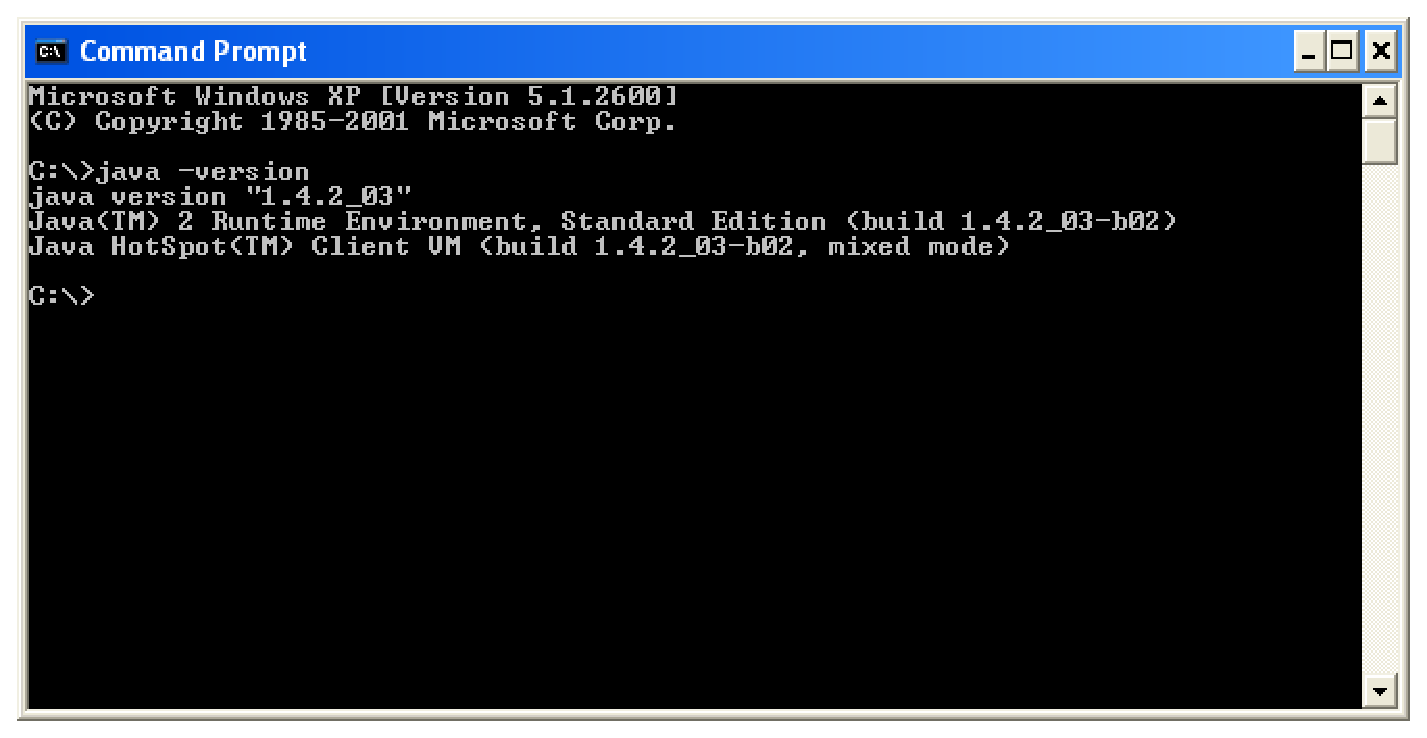
\includegraphics[width=5.0in]{UserManualInputs/images/install.eps}
        \caption{V�rification de la version de la machine virtuelle Java}\label{install}
      \end{center}
 \end{figure}

S'il n'y a pas de machine virtuelle Java install�e sur l'ordinateur,
il faut t�l�charger la derni�re version disponible sur la page de
t�l�chargement en cliquant sur le lien \verb!j2re-1.5.0_01.exe! et
effectuer l'installation.

Si la machine virtuelle Java install�e sur l'ordinateur est
ant�rieure � la \verb!version 1.5.0_01!, il faut d'abord
d�sinstaller l'ancienne version, puis t�l�charger la plus r�cente
disponible sur la page de t�l�chargement en cliquant sur le lien
\verb!j2re-1.5.0_01.exe! et enfin effectuer l'installation.

Une fois assur� de la bonne version de la machine virtuelle Java, l'installation de \dx{} peut commencer.

\begin{enumerate}
    \item T�l�charger \dx{} en cliquant sur \verb!tictac.zip! � partir de la page de t�l�chargement puis ouvrir le fichier ;
    \item Extraire le contenu du fichier \verb!tictac.zip! vers l'emplacement de votre choix (sur votre disque, \verb!C:\! par exemple).
\end{enumerate}

L'installation �tant termin�e, vous pouvez commencer � utiliser
\dx{}. Pour lancer l'application, double-cliquez sur le fichier
\verb!Diamant.bat! se trouvant dans le dossier d'installation \dx{}
(c'est-�-dire l'emplacement choisi pour le contenu du fichier
\verb!tictac.zip!).

\section{Mise � jour}

La mise � jour de \dx{} peut se faire de deux fa�ons:
\begin{itemize}
    \item Si la nouvelle version disponible sur la page de t�l�chargement du site web est un fichier \verb!.zip!:
    \begin{enumerate}
            \item T�l�charger \dx{} en cliquant sur \verb!tictac.zip! � partir de la page de t�l�chargement puis ouvrir le fichier;
            \item Extraire le contenu du fichier \verb!tictac.zip! dans le dossier d'installation de \dx{}.
    \end{enumerate}

    \item Si la nouvelle version disponible sur la page de t�l�chargement du site web est le fichier \verb!tictac.jar!, t�l�chargez ce fichier en cliquant sur \verb!tictac.jar! et enregistrez-le dans le dossier d'installation de \dx{} (dans notre exemple, il s'agit du dossier \verb!C:\!\dx{}).
\end{itemize}

\chapter{Modification de la grille horaire}\label{grille}
\section{Introduction}\ \label{horaire}
Construire un horaire avec \dx{} passe d'abord par le chargement d'une grille horaire. Cette grille horaire peut �tre pr�alablement modifi�e afin qu'elle s'adapte mieux � vos besoins du moment. La grille horaire est d�finie dans un fichier portant l'extension \emph{.xml}) et elle peut �tre modifi�e � partir d'une interface avec barre de t�ches pour rendre les fonctions suivantes:

\begin{itemize}
    \item Ajout et/ou suppression de jours, modification du nom d'une journ�e;
    \item Modification de la priorit� d'une p�riode;
\end{itemize}

Nous vous pr�senterons en detail, dans les prochaines sections, la proc�dure de chargement de la grille horaire en mode modification, ainsi que les diff�rentes fonctions permettant de la modifier.

\section{Chargement de la grille horaire} 
\begin{enumerate}
    \item Lancer \dx{}. Une fois \dx{} lanc�, le chargement de la grille peut se faire de deux fa�ons.
        \begin{figure}[h]
      % Requires \usepackage{graphicx}
          \begin{center}
            \includegraphics[width=4.2in]{UserManualInputs/images/grilleModif.eps}
            \caption{Grille horaire}\label{grillecycModif}
          \end{center}
        \end{figure}
        
    \item Chargement de la grille:
    \begin{itemize}
        \item Chargement d'une nouvelle grille. Le chargement se fait � partir de la grille par d�faut poss�dant la configuration standard. Pour cela, allez au menu \textbf{\emph{Fichier}} \Rar \textbf{\emph{Nouvel grille}} \Rar \textbf{\emph{Grille cycle}} ou \textbf{\emph{Grille examen}} (selon le besoin), la grille horaire par d�faut est charg�e et pr�sent�e � l'�cran (voir figure \ref{grillecycModif}).
        \item Ouverture d'une grille existante. Pour ouvrir une grille existante, Allez au menu \textbf{\emph{Fichier}} \Rar \textbf{\emph{Ouvrir grille}}\index{Fichier \Rar Ouvrir} Une bo�te de dialogue comme celle de la Figure \ref{selectgrillemodif} doit appara�tre et elle vous permettra de choisir le fichier (fichier avec extension \emph{.xml}) contenant la d�finition de votre grille horaire. En cliquant sur le bouton \emph{\textbf{Grille horaire}}, la grille horaire s�lectionn�e est charg�e et pr�sent�e � l'�cran (voir figure \ref{grillecycModif})
                
    \begin{figure}[h]
    % Requires \usepackage{graphicx}
    \begin{center}
        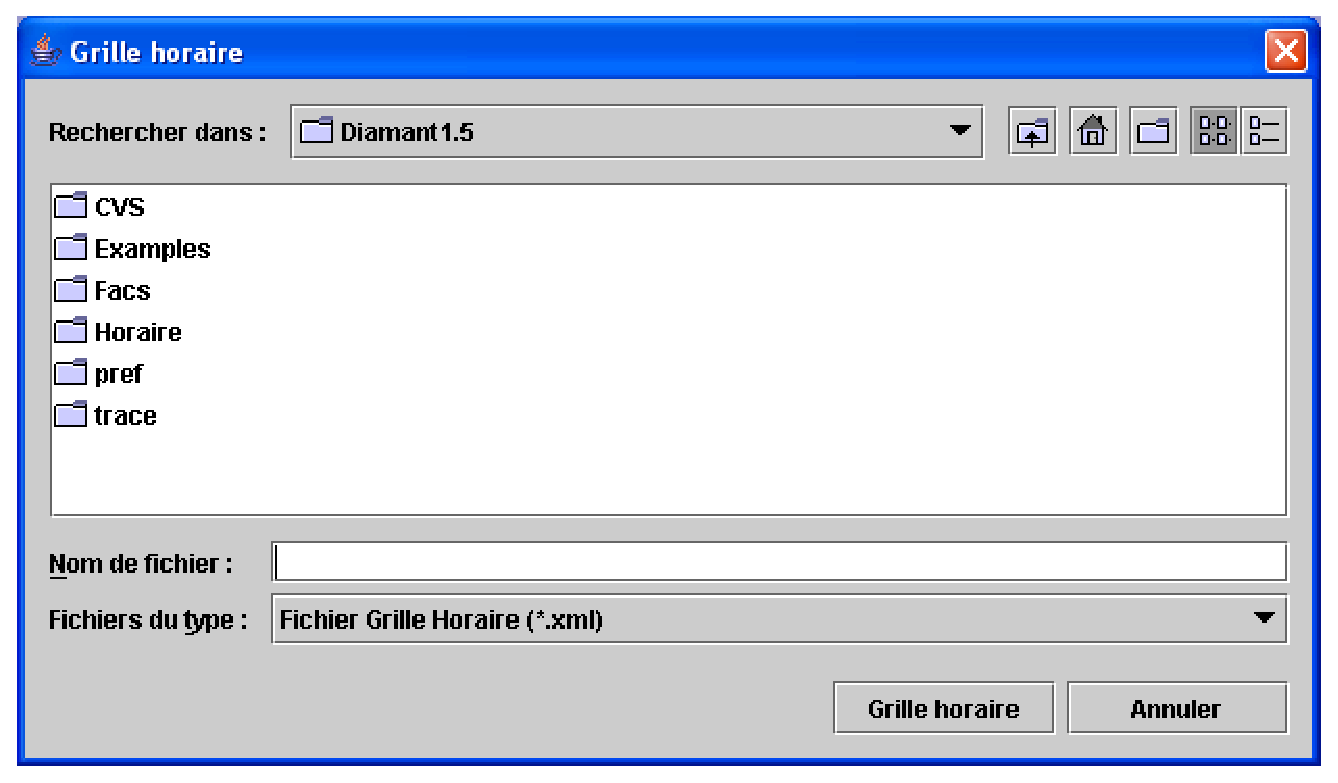
\includegraphics[width=3.5in]{UserManualInputs/images/selectXMLfileModif.eps}
        \caption{Selection de la grille horaire}\label{selectgrillemodif}
    \end{center}
    \end{figure}
    
    \end{itemize}        
    
\end{enumerate}

\section{Ajout et/ou suppression de jours, modification du nom d'une journ�e}

Ces fonctions sont r�alis�es � partir de la barre de t�ches de gestion de journ�es de la figure \ref{toolbarday}, obtenue en s�lectionnant \emph{\textbf{Jour}} � partir de la barre de t�che.

    \begin{figure}[h]
    % Requires \usepackage{graphicx}
        \begin{center}
            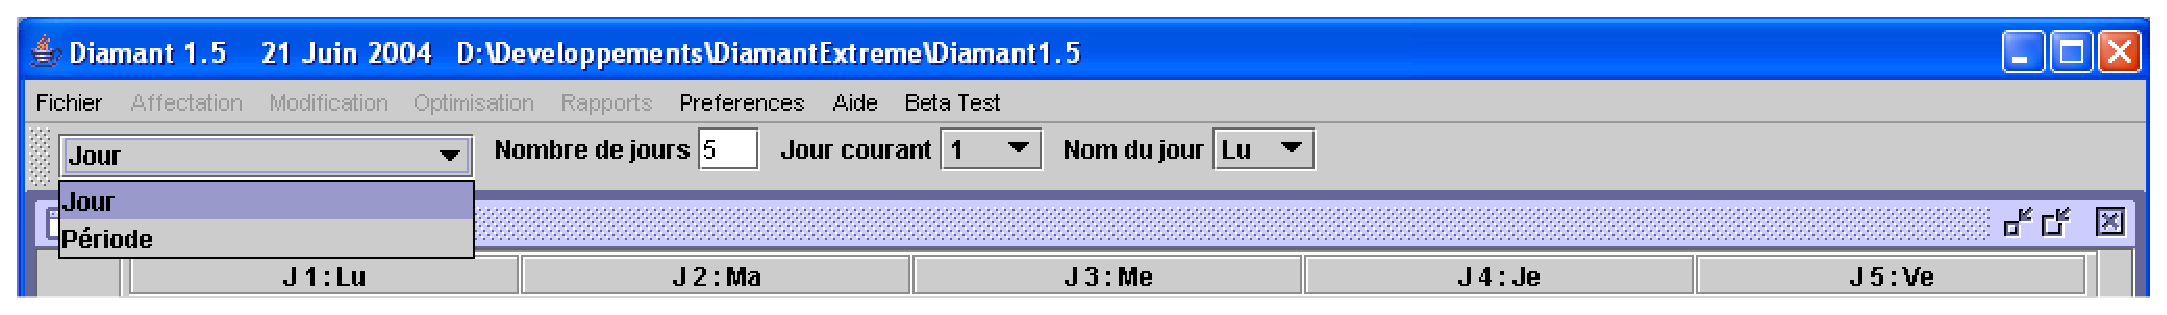
\includegraphics[width=6.0in]{UserManualInputs/images/toolbar_day.eps}
            \caption{Barre de t�ches de gestion de journ�es}\label{toolbarday}
        \end{center}
    \end{figure}
    
\subsection{Ajout et/ou suppression de jours}

Pour ajouter ou supprimer des jours, il suffit d'entrer dans la zone \emph{\textbf{Nombre de jours}} de la barre de t�che, le nombre de jours que vous souhaitez obtenir et le valider en appuyant sur la touche \textbf{\emph{Entrer}}. En fonction du nombre de jours courant, \dx{} ajoutera ou supprimera des jours.

        \begin{figure}[h]
        % Requires \usepackage{graphicx}
            \begin{center}
                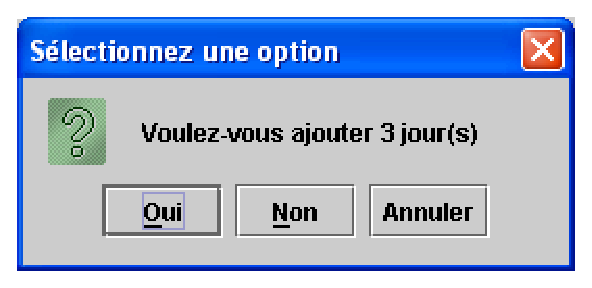
\includegraphics[width=2.0in]{UserManualInputs/images/addDays.eps}
                \caption{Confirmation d'ajout de jours}\label{addDays}
            \end{center}
        \end{figure}

 \begin{description}
    \item[Exemple 1:]  Si le nombre de jours courant est 7 et que l'on d�sire avoir 10 jours, le syst�me vous demandera si vous voulez ajouter 3 jours (voir figure \ref{addDays}).
        
        \item[Exemple 2:]  Si le nombre de jours courant est 7 et que l'on d�sire avoir 5 jours, le syst�me vous demandera si vous voulez supprimer 2 jours (voir figure \ref{remDays}).
        \begin{figure}[h]
        % Requires \usepackage{graphicx}
            \begin{center}
                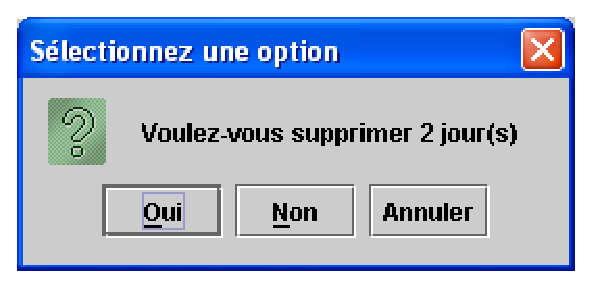
\includegraphics[width=2.0in]{UserManualInputs/images/remDays.eps}
                \caption{Confirmation de suppression de jours}\label{remDays}
            \end{center}
        \end{figure}

\end{description}     

\subsection{Modification du nom d'une journ�e}

� partir de la barre de t�ches (figure \ref{toolbarday}), s�lectionnez l'index du jour auquel l'on souhaite modifier le nom, � l'aide de la liste d�roulante de la zone \emph{\textbf{Jour courant}} ; s�lectionnez ensuite le nom du jour � l'aide de la liste d�roulante de la zone \emph{\textbf{Nom du jour}}; les changements seront instantan�ment refl�t�s sur la grille horaire.

\section{Modification de la priorit� d'une p�riode}

Ces fonctions sont r�alis�es � partir de la barre de t�ches de gestion de p�riodes de la figure \ref{toolbarper}, obtenue en s�lectionnant \emph{\textbf{P�riode}} � partir de la barre de t�che.

    \begin{figure}[h]
    % Requires \usepackage{graphicx}
        \begin{center}
            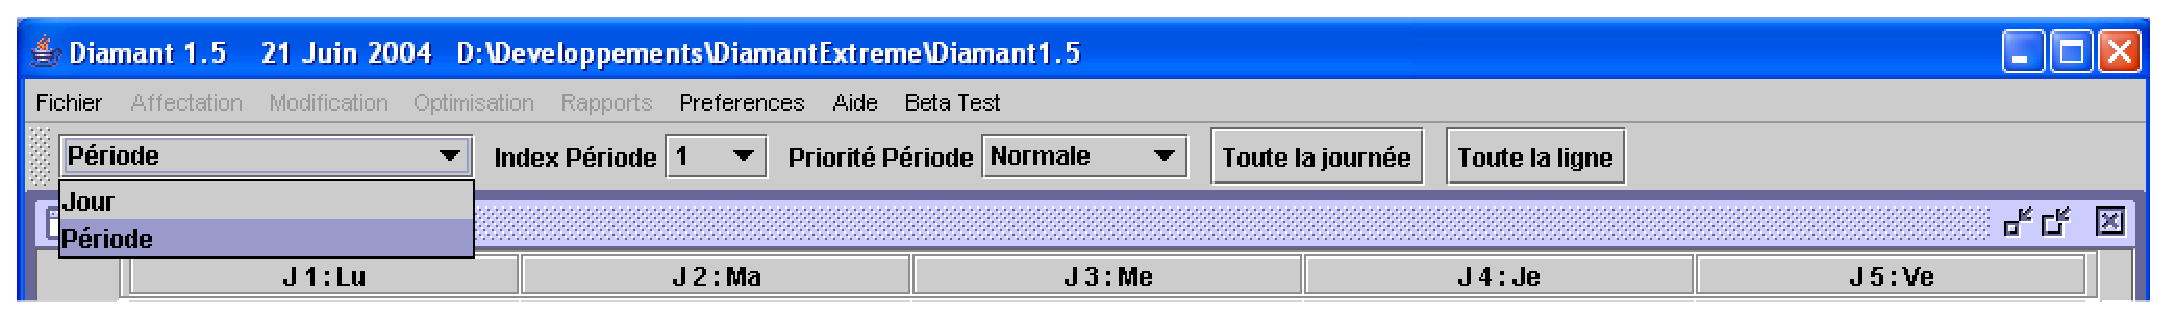
\includegraphics[width=6.0in]{UserManualInputs/images/toolbar_period.eps}
            \caption{Barre de t�ches de gestion de p�riodes}\label{toolbarper}
        \end{center}
    \end{figure}
    
Pour modifier la priorit� d'une p�riode, proc�dez comme suit:

\begin{enumerate}
    \item S�lectionnez la p�riode � modifier.
   \begin{itemize}
    \item S�lectionnez l'index de la p�riode sur la barre de t�ches � l'aide de la liste d�roulante de la zone \emph{\textbf{Index P�riode}}; \\
    \textbf{ou}
    \item S�lectionnez la p�riode en cliquant simplement sur la p�riode sur la grille horaire.
\end{itemize}  
 
    \item S�lectionnez la priorit� � l'aide de la liste d�roulante de la zone \emph{\textbf{Priorit� P�riode}} et les changements seront instantan�ment refl�t�s sur la grille horaire.
    \item L'op�ration faite sur une p�riode peut �tre appliqu�e � toutes les autres p�riodes de la m�me journ�e en cliquant sur le bouton \emph{\textbf{Toute la journ�e}} de la barre de t�ches, elle peut �galement �tre appliqu�e � toutes les autres p�riodes de la m�me ligne (c'est � dire toutes les autres p�riodes commen�ant � la m�me heure) en cliquant sur le bouton \emph{\textbf{Toute la ligne}} de la barre de t�ches.
\end{enumerate}    

\chapter{Construction d'un horaire avec \dx{}}

Construire un horaire avec \dx{} laisse supposer que l'utilisateur
a d�j� sur son ordinateur les fichiers n�cessaires (ceux du STI et
ceux de la Facult�)~: cours.sig, choixet.sig, disprof.sig et
locaux.txt. Ces fichiers peuvent porter n'importe quel nom, mais
pour notre exemple, les noms sont bien explicites. Il est
conseill� de regrouper toutes les informations concernant les
horaires d'un trimestre dans un r�pertoire (par exemple hiver04 ou
h2004). Ainsi, les fichiers d'importation et les fichiers produits
pendant la construction d'un horaire seront ensemble.

La construction d'un nouvel horaire avec \dx{} comporte trois principales �tapes. Elle d�bute par une
phase de pr�paration (phase 1), se poursuit par une phase de modification et d'�puration des donn�es (phase 2) et se termine par la construction � proprement parler (phase 3). La construction de l'horaire peut se poursuivre au del� de la phase 3, par l'utilisation d'outils permettant de raffiner l'horaire (Affectation manuelle, rapports, etc).

Nous vous pr�senterons dans ce chapitre les phases de
pr�paration d'un horaire avec \dx{}, de modification et d'�puration des donn�es, les
caract�ristiques particuli�res de la construction d'un horaire de
cours et d'un horaire d'examen, et nous terminerons les outils de raffinement de l'horaire. Toutefois, les options du logiciel ne seront pas toutes pr�sent�es.

\section{Production d'un horaire de cours}

\subsection{Pr�paration de l'horaire}\label{finprepa}

\begin{enumerate}
    \item Lancer \dx{}.
    \item Aller au menu \textbf{\emph{Fichier}},
    puis s�lectionner le menu \textbf{\emph{Nouvel horaire}}
    et enfin s�lectionner le sous-menu \textbf{\emph{Horaire cycle}}.
    Une bo�te de dialogue comme celle
de la Figure \ref{selectgrillecyc} doit appara�tre et elle vous
permettra de choisir le fichier (fichier avec extension \emph{.xml})
contenant la d�finition de votre grille horaire.

    \begin{figure}[h]
    % Requires \usepackage{graphicx}
    \begin{center}
        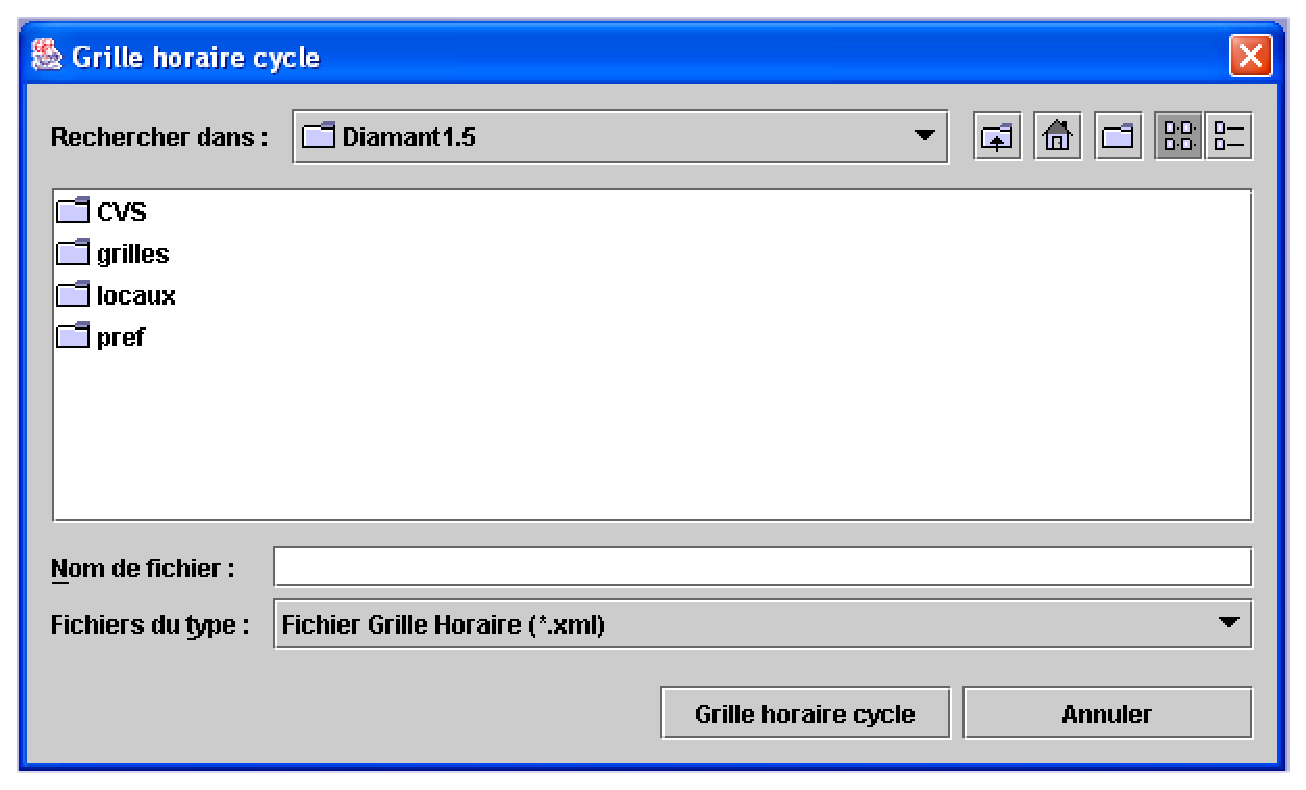
\includegraphics[width=2.5in]{UserManualInputs/images/selectXMLfile.eps}
        \caption{Selection de la grille horaire de cours}\label{selectgrillecyc}
    \end{center}
    \end{figure}

    \item En cliquant sur le bouton \emph{\textbf{OK}}, la grille horaire s�lectionn�e est charg�e et pr�sent�e � l'�cran (voir figure \ref{grillecyc}).
\begin{figure}[h]
  % Requires \usepackage{graphicx}
  \begin{center}
    \includegraphics[width=4.5in]{UserManualInputs/images/grille.eps}
    \caption{Grille horaire de cours}\label{grillecyc}
  \end{center}
\end{figure}

    \item Aller au menu \textbf{\emph{Fichier}} et s�lectionner le menu \textbf{\emph{D�finir fichiers � importer}}. Une bo�te de dialogue comme celle de la Figure \ref{defautoimport}  doit appara�tre. Rep�rer l'endroit o� chacun des fichiers est localis�, puis cliquer sur le bouton \textbf{\emph{OK}}. Une nouvelle fen�tre se pr�sentera afin de vous permettre d'enregistrer la configuration des fichiers que vous venez de faire.

Il est recommand� d'enregistrer cette configuration en utilisant un nom de fichier unique et repr�sentatif.

Exemple: choisissez le nom de fichier \emph{E02cours} pour \emph{�t� 2002 horaire de cours} et le fichier cr�� sera \emph{E02cours.dim}. L'extension \textbf{\emph{.dim}} est rajout� automatiquement.

\begin{figure}[h]
  % Requires \usepackage{graphicx}
  \begin{center}
    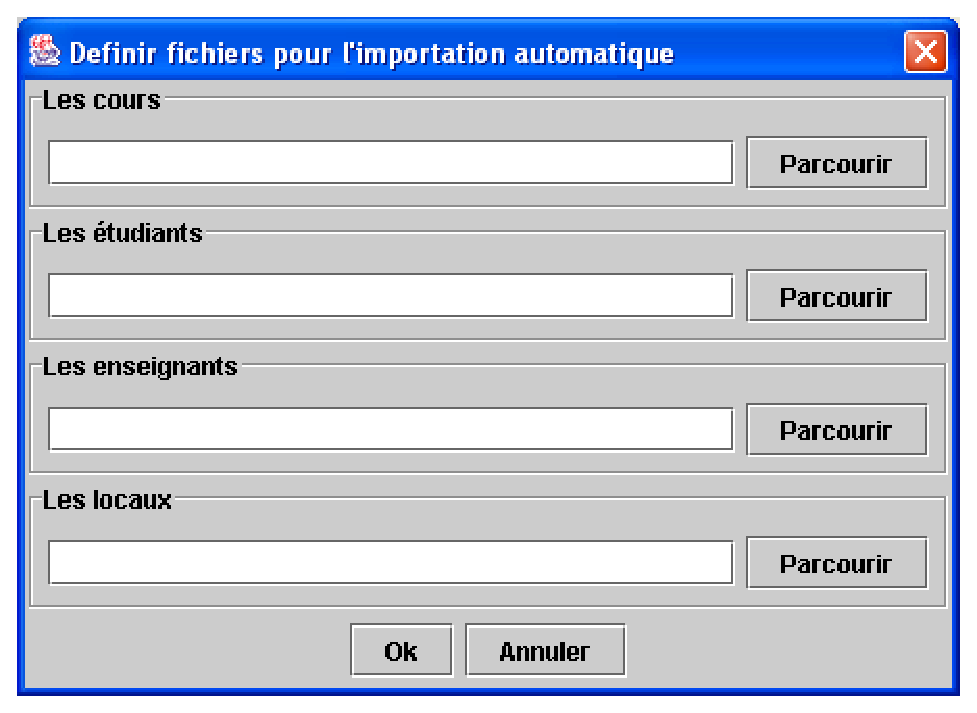
\includegraphics[width=2.5in]{UserManualInputs/images/autoimport.eps}
    \caption{D�finition des fichiers d'importation}\label{defautoimport}
  \end{center}
\end{figure}

    \item Aller au menu \textbf{\emph{Fichier}} et s�lectionner le menu \textbf{\emph{Importer automatiquement}}.
    Une boite de dialogue appara�tra et vous permettra de choisir le fichier \textbf{\emph{.dim}} de �configuration de fichiers�
    pr�c�demment cr�� � partir de la fonction  \textbf{\emph{D�finir fichiers � importer}}
    (dans l'exemple pr�c�dent il s'agit du fichier \emph{E02cours.dim}).
    Cliquer � pr�sent sur le bouton \textbf{\emph{Importation de fichiers}},
    toutes vos donn�es (cours, �tudiants, enseignants et locaux) seront charg�es dans le logiciel et
    pr�tes � �tre modifi�es.
\end{enumerate}

� partir de cette �tape, la construction de l'horaire � proprement parler peut commencer. Il est vivement recommand� de lancer l'\textbf{\emph{affectation initiale}} � partir du menu \textbf{\emph{Optimisation}} avant de poursuivre la production de l'horaire. Lancer l'\textbf{\emph{affectation initiale}} � cette �tape ex�cuterait les fonctionnalit�s suivantes:

\begin{enumerate}
    \item Placer de fa�on al�atoire dans les groupes d'activit�, les �tudiants non pr�-affect�s � des groupes, tout en �quilibrant les groupes.
    \item Placer les �v�nements pr�-affect�s (plac�s ou fig�s) dans la grille horaire.
    \item Calculer les conflits g�n�r�s.
\end{enumerate}

Cette affectation initiale permettrait donc d'initialiser le logiciel de sorte � pouvoir faire des modifications sur les donn�es et observer imm�diatement les repercussions sur l'horaire.

La pr�paration de l'horaire �tant achev�e, nous pouvons � pr�sent passer � la phase de modification et d'�puration de donn�es (phase 2). Il est cependant n�cessaire de noter que cette phase peut avoir lieu avant ou apr�s la phase de construction � proprement parler (phase 3), mais nous recommandons de la faire avant la phase 3 afin de travailler une bonne fois pour toute sur des donn�es propres (�pur�es).

\subsection{Modification et �purations des donn�es}

Le but de cette �tape est de permettre de construire l'horaire uniquement � partir de donn�es propres. Cette modification et/ou �puration peut se faire sur les activit�s, les �v�nements, les groupes d'�tudiants, les enseignants ou les locaux. 

\begin{itemize}
    \item Modifier une activit� en cliquant sur le menu \textbf{\emph{Affectation}} et le sous menu \textbf{\emph{Activit�s}} pour voir appara�tre la \emph{liste des activit�s} (voir figure \ref{listactc}) ou alors cliquer sur le menu \textbf{\emph{Affectation}} et le sous menu \textbf{\emph{�v�nements}} pour voir appara�tre la \emph{liste des �v�nements} (voir figure \ref{listeeventc}).\\

� partir de la fen�tre \emph{liste des �v�nements}, vous pouvez s�lectionner un ou plusieurs �v�nements et les faire passer de la colonne \emph{fig�s} (les �v�nements sont plac�es et fig�es dans la grille horaire) � \emph{plac�s} (les �v�nements sont plac�es dans la grille horaire) ou de la colonne \emph{plac�s} � \emph{non plac�s} (les �v�nements ne sont pas encore plac�es dans la grille horaire) et vice-versa. 

    \begin{figure}[h]
      % Requires \usepackage{graphicx}
      \begin{center}
        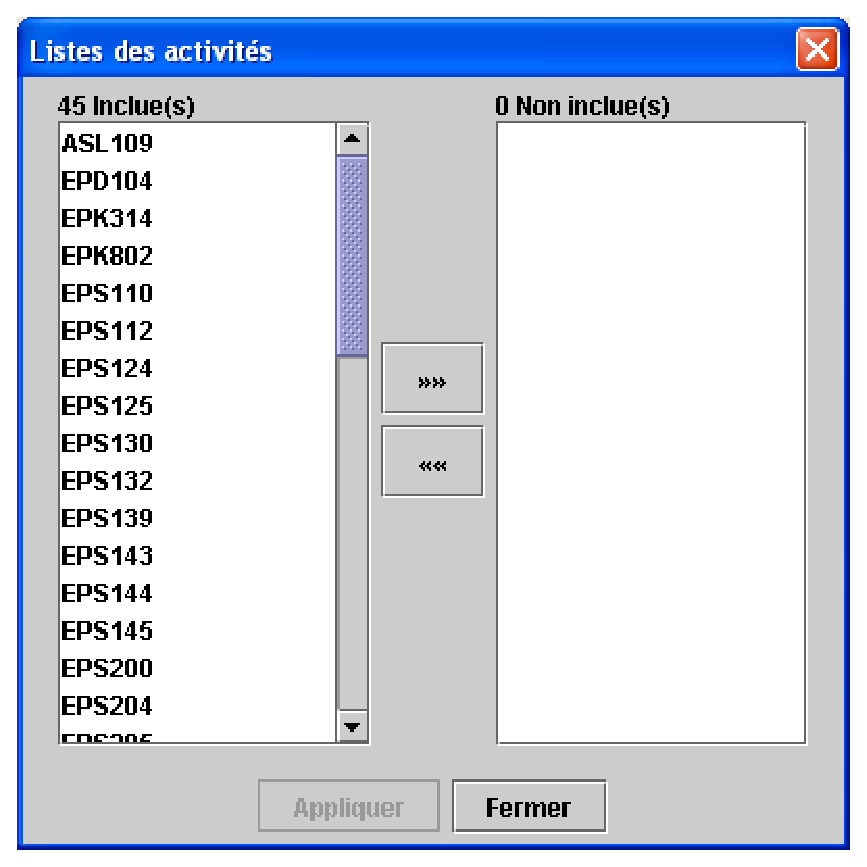
\includegraphics[width=2.5in]{UserManualInputs/images/listeact.eps}
        \caption{Liste des activit�s}\label{listactc}
      \end{center}
    \end{figure}

� partir de la fen�tre \emph{liste des activit�s}, vous pouvez s�lectionner une ou plusieurs activit�s et les faire passer de la colonne \emph{inclue(s)} � \emph{non inclue(s)} (non inclue(s)= les activit�s ne seront pas utilis�es dans la construction de l'horaire) et vice-versa. \\

    \begin{figure}[h]
      % Requires \usepackage{graphicx}
      \begin{center}
        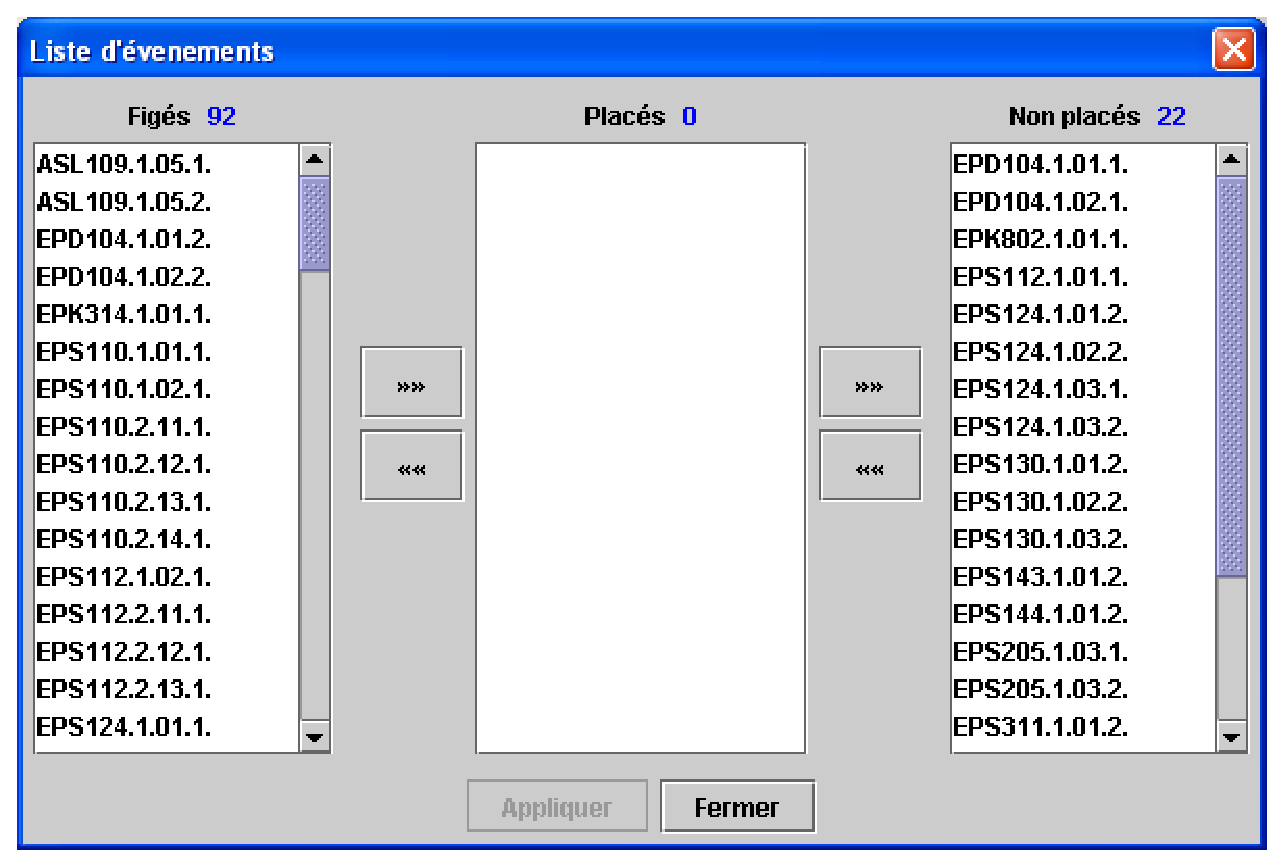
\includegraphics[width=2.5in]{UserManualInputs/images/listeevent.eps}
        \caption{Liste des �v�nements}\label{listeeventc}
      \end{center}
    \end{figure}
   

� partir de l'une ou l'autre des fen�tres, double-cliquer sur l'activit� ou l'�v�nement � modifier pour faire appara�tre le dialogue d'\emph{affectation d'�v�nements} (voir figure \ref{eventc}). Il vous est possible de modifier, � partir de cette fen�tre d'\emph{affectation d'�v�nements}, le jour et l'heure de d�but de l'�v�nement, l'enseignant, le local, de placer ou figer l'activit�.

    \begin{figure}[h]
      % Requires \usepackage{graphicx}
      \begin{center}
        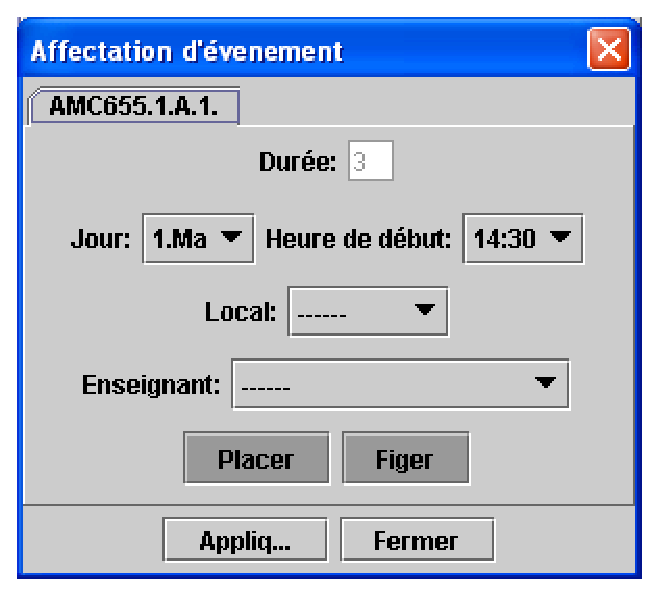
\includegraphics[width=2.5in]{UserManualInputs/images/event.eps}
        \caption{Affectation d'�v�nement}\label{eventc}
      \end{center}
    \end{figure}
    
Cliquer sur \textbf{\emph{Appliquer}} pour valider les changements et Cliquer sur \textbf{\emph{Fermer}} pour fermer la fen�tre.\\
    
    \item Ajouter ou supprimer un groupe ou un �v�nement en cliquant sur le menu \textbf{\emph{Modification}} et le sous menu \textbf{\emph{Activit�}} pour voir appara�tre la fen�tre d'\textbf{\emph{Activit�s}} de la figure \ref{modifactc}.

    \begin{figure}[h]
      % Requires \usepackage{graphicx}
      \begin{center}
        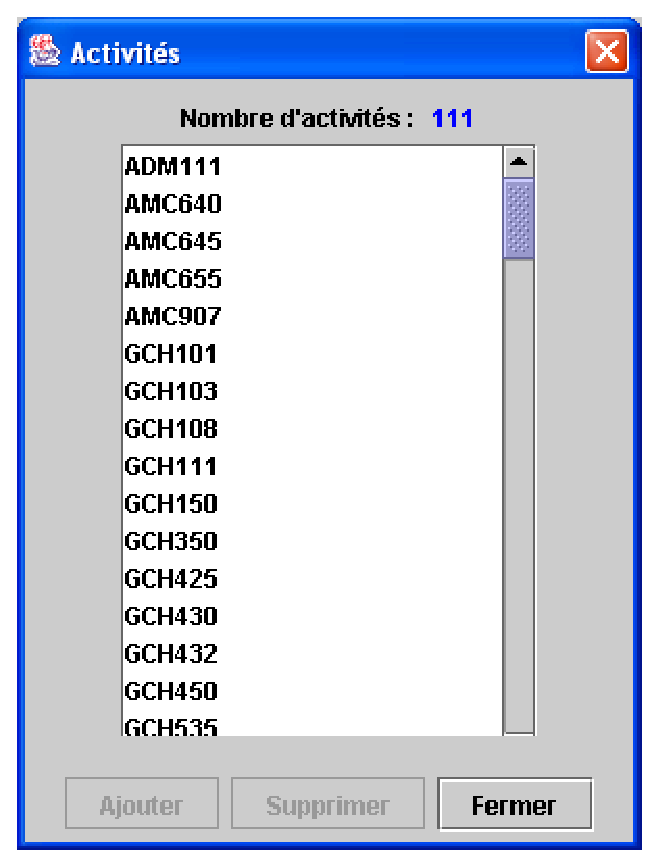
\includegraphics[width=2.5in]{UserManualInputs/images/modifact.eps}
        \caption{Modification d'activit�s}\label{modifactc}
      \end{center}
    \end{figure}

Double-cliquer sur l'activit� que vous souhaitez modifier pour voir appara�tre la fen�tre de \textbf{\emph{Natures}} de la figure \ref{modiftypec}.

    \begin{figure}[h]
      % Requires \usepackage{graphicx}
      \begin{center}
        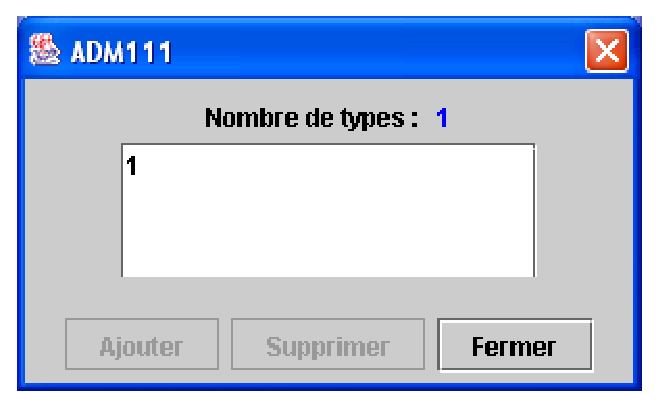
\includegraphics[width=2.5in]{UserManualInputs/images/modiftype.eps}
        \caption{Modification de natures}\label{modiftypec}
      \end{center}
    \end{figure}

Double-cliquer sur la nature que vous souhaitez modifier pour voir appara�tre la fen�tre de \textbf{\emph{Groupes)}} de la figure \ref{modifgroupec}.

    \begin{figure}[h]
      % Requires \usepackage{graphicx}
      \begin{center}
        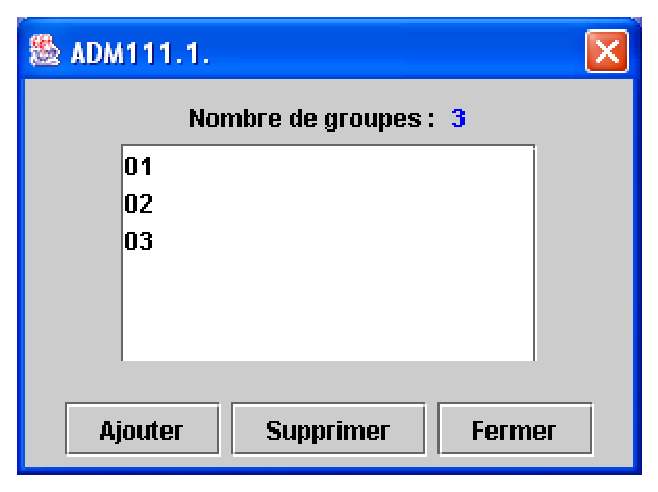
\includegraphics[width=2.5in]{UserManualInputs/images/modifgroupe.eps}
        \caption{Modification de groupe}\label{modifgroupec}
      \end{center}
    \end{figure}
� partir de cette fen�tre, vous avez trois possibilit�s:
        \begin{enumerate}
            \item Cliquer sur le bouton \textbf{\emph{Ajouter}}, pour ajouter un groupe. Le groupe sera ajout� � la suite du dernier groupe de la liste.
            \item Cliquer sur le bouton \textbf{\emph{Supprimer}}, pour supprimer un groupe. Le dernier groupe de la liste sera supprim�.
            \item Double-cliquer sur le groupe que vous souhaitez modifier pour voir appara�tre la fen�tre d'\textbf{\emph{�v�nements}} de la figure \ref{modifunitc}. � partir de cette fen�tre, pour pouvez ajouter, supprimer ou modifier un �v�nement.

    \begin{figure}[h]
      % Requires \usepackage{graphicx}
      \begin{center}
        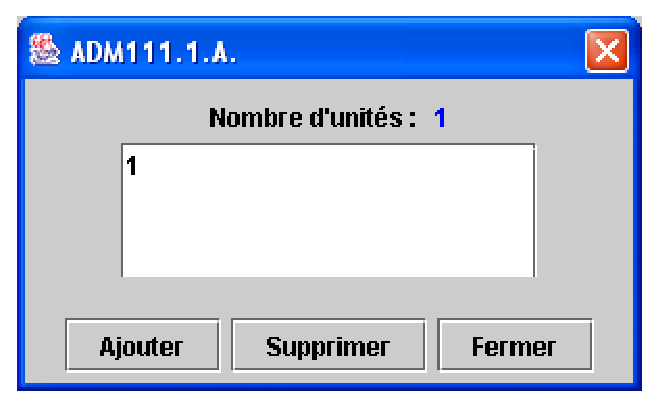
\includegraphics[width=2.5in]{UserManualInputs/images/modifunit.eps}
        \caption{Modification d'�v�nements}\label{modifunitc}
      \end{center}
    \end{figure}
            
            Double-cliquer sur l'�v�nement que vous souhaitez modifier pour voir appara�tre la fen�tre d'\emph{affectation d'�v�nements} (voir figure \ref{eventc}). Il sera possible de faire, dans cette fen�tre, toutes les modifications d�crites pr�c�demment; il �galement possible de modifier la dur�e d'un �v�nement.
        \end{enumerate}    

\item Modifier les groupes d'�tudiants en cliquant sur le menu \textbf{\emph{Affectation}} et le sous menu \textbf{\emph{Groupes}} pour voir appara�tre la fen�tre de la figure \ref{groupec}. S�lectionner dans la colonne de droite (�tudiants assign�s) le groupe (Groupe A, Groupe B, ...) que l'on souhaite modifier. S�lectionner ensuite un ou plusieurs �tudiants que l'on souhaite d�placer. Utilisez enfin les fl�ches pour d�placer les �tudiants de la gauche vers la droite ou vice-versa.

    \begin{figure}[h]
      % Requires \usepackage{graphicx}
      \begin{center}
        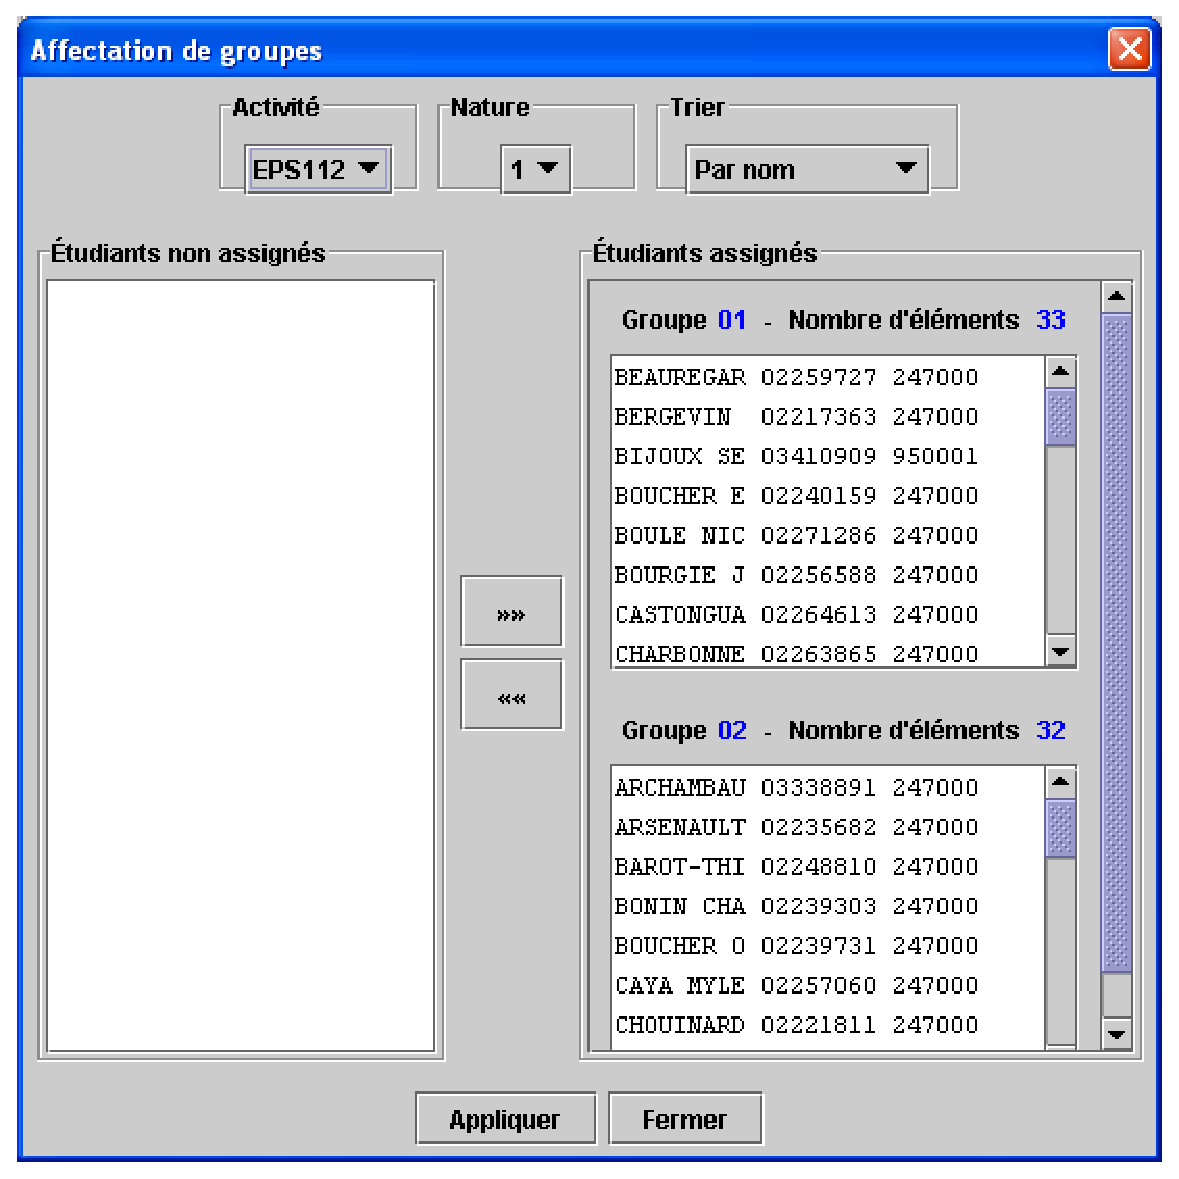
\includegraphics[width=2.5in]{UserManualInputs/images/groupe.eps}
        \caption{Affectation des groupes}\label{groupec}
      \end{center}
    \end{figure}

Cliquer sur le bouton \textbf{\emph{Par matricule/Par programme/Par nom}} dans le zone \emph{trier}, pour trier les �tudiants par matricule, par programme ou par nom.

Cliquer sur \textbf{\emph{Appliquer}} pour valider les changements et Cliquer sur \textbf{\emph{Ok}} pour valider les changements et fermer la fen�tre.\\

\item Modifier la disponibilit� d'un enseignant en cliquant sur le menu \textbf{\emph{Affectation}} et le sous menu \textbf{\emph{Enseignants}} pour voir appara�tre la fen�tre de la figure \ref{enseignantc}. En s�lectionnant une zone correspondant au jour et � l'heure que vous souhaitez modifier. Une zone s�lectionn�e appara�t en fonc� et indique que l'enseignant y est disponible.
 
    \begin{figure}[h]
      % Requires \usepackage{graphicx}
      \begin{center}
        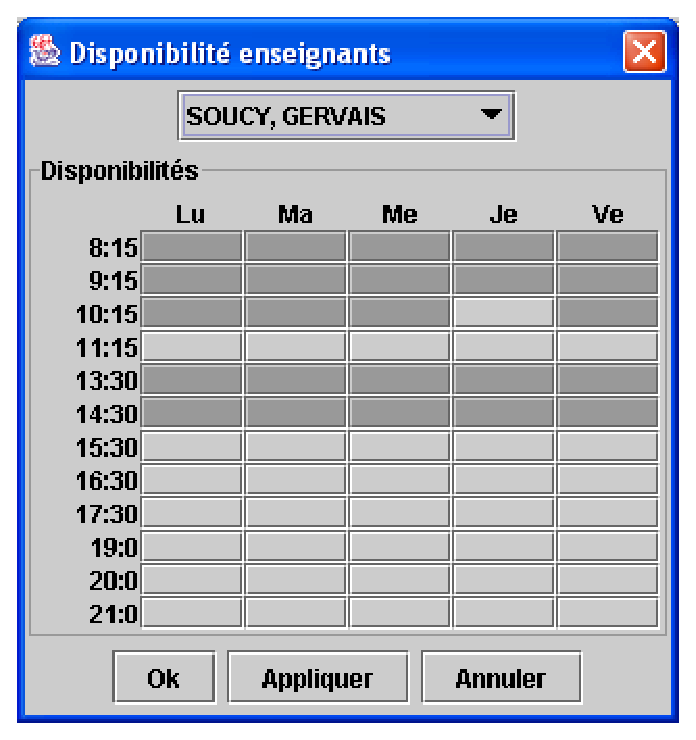
\includegraphics[width=2.5in]{UserManualInputs/images/enseignant.eps}
        \caption{Disponibilit� des enseignants}\label{enseignantc}
      \end{center}
    \end{figure}

Cliquer sur \textbf{\emph{Appliquer}} pour accepter et effectuer les changements et Cliquer sur \textbf{\emph{Ok}} pour accepter, effectuer les changements et fermer la fen�tre.    \\

    \item Modifier la disponibilit� d'un local en cliquant sur le menu \textbf{\emph{Affectation}} et le sous menu \textbf{\emph{Locaux}} pour voir appara�tre la fen�tre de la figure  \ref{localc}. En s�lectionnant une zone correspondant au jour et � l'heure que vous souhait� modifier. Une zone s�lectionn�e appara�t en fonc� et indique que le local y est disponible. 

    \begin{figure}[h]
      % Requires \usepackage{graphicx}
      \begin{center}
        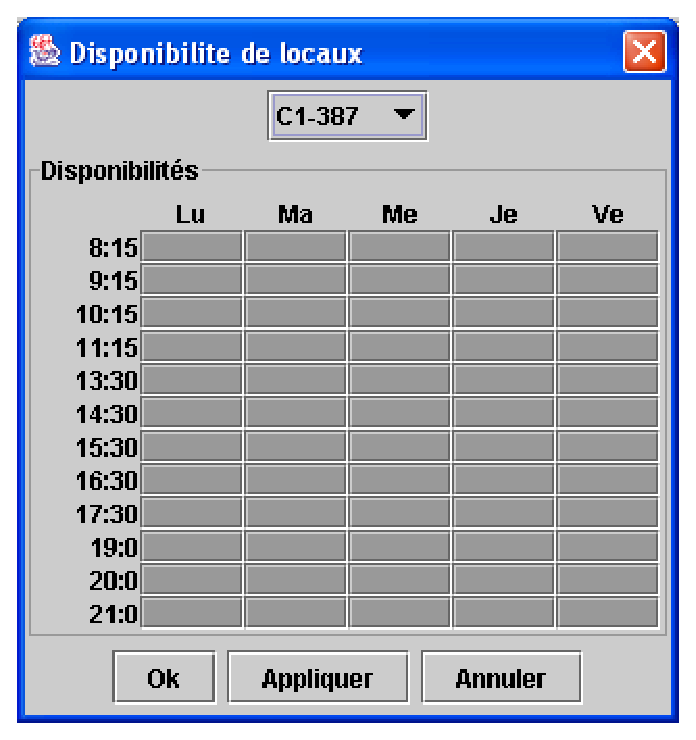
\includegraphics[width=2.5in]{UserManualInputs/images/local.eps}
        \caption{Disponibilit� des locaux}\label{localc}
      \end{center}
    \end{figure}

Cliquer sur \textbf{\emph{Appliquer}} pour accepter et effectuer les changements et Cliquer sur \textbf{\emph{Ok}} pour accepter, effectuer les changements et fermer la fen�tre.\\
        
 \end{itemize}    

\subsection{Construction de l'horaire}

\subsubsection{Affectation des �v�nements}

Il est vivement recommand� de commencer cette �tape en lan�ant l'\textbf{\emph{affectation initiale}} � partir du menu \textbf{\emph{Optimisation}} (si cela n'a pas �t� pr�c�demment fait � la fin de la phase de pr�paration de l'horaire - section \ref{finprepa}) avant de poursuivre la production de l'horaire.

L'\emph{affectation initiale} a pour but d'ex�cuter les commandes suivantes :

\begin{enumerate}
    \item Placer de fa�on al�atoire dans les groupes d'activit�, les �tudiants non pr�-affect�s � des groupes, tout en �quilibrant les groupes.
    \item Placer les �v�nements pr�-affect�s (plac�s ou fig�s) dans la grille horaire.
    \item Calculer les conflits g�n�r�s.
\end{enumerate}  

Une fois l'affectation initiale effectu�e, l'�tape suivante consiste � lancer le sous menu \textbf{\emph{Construire l'horaire}} � partir du menu \textbf{\emph{Optimisation}}, afin de laisser le logiciel placer automatiquement dans la grille horaire les �v�nements (ceux qui n'ont pas encore �t� plac�s dans la grille horaire) respectant toutes les contraintes sp�cifi�es et ne cr�ant aucun nouveau conflit (conflits d'enseignants, conflits d'�tudiants et conflits de locaux).

\subsubsection{Raffinement de l'horaire}


\section{Production d'un horaire d'examen}

\subsection{Pr�paration de l'horaire}\label{finprepae}

\begin{enumerate}
    \item Lancer \dx{}.
    \item Aller au menu \textbf{\emph{Fichier}},
    puis s�lectionner le menu \textbf{\emph{Nouvel horaire}}
    et enfin s�lectionner le sous-menu \textbf{\emph{Horaire Examen}}.
    Une bo�te de dialogue comme celle
de la Figure \ref{selectgrillecyc} doit appara�tre et elle vous
permettra de choisir le fichier (fichier avec extension \emph{.xml})
contenant la d�finition de votre grille horaire.

    \item En cliquant sur le bouton \emph{\textbf{OK}}, la grille horaire s�lectionn�e est charg�e et pr�sent�e � l'�cran (voir figure \ref{grilleexam}).
\begin{figure}[h]
  % Requires \usepackage{graphicx}
  \begin{center}
    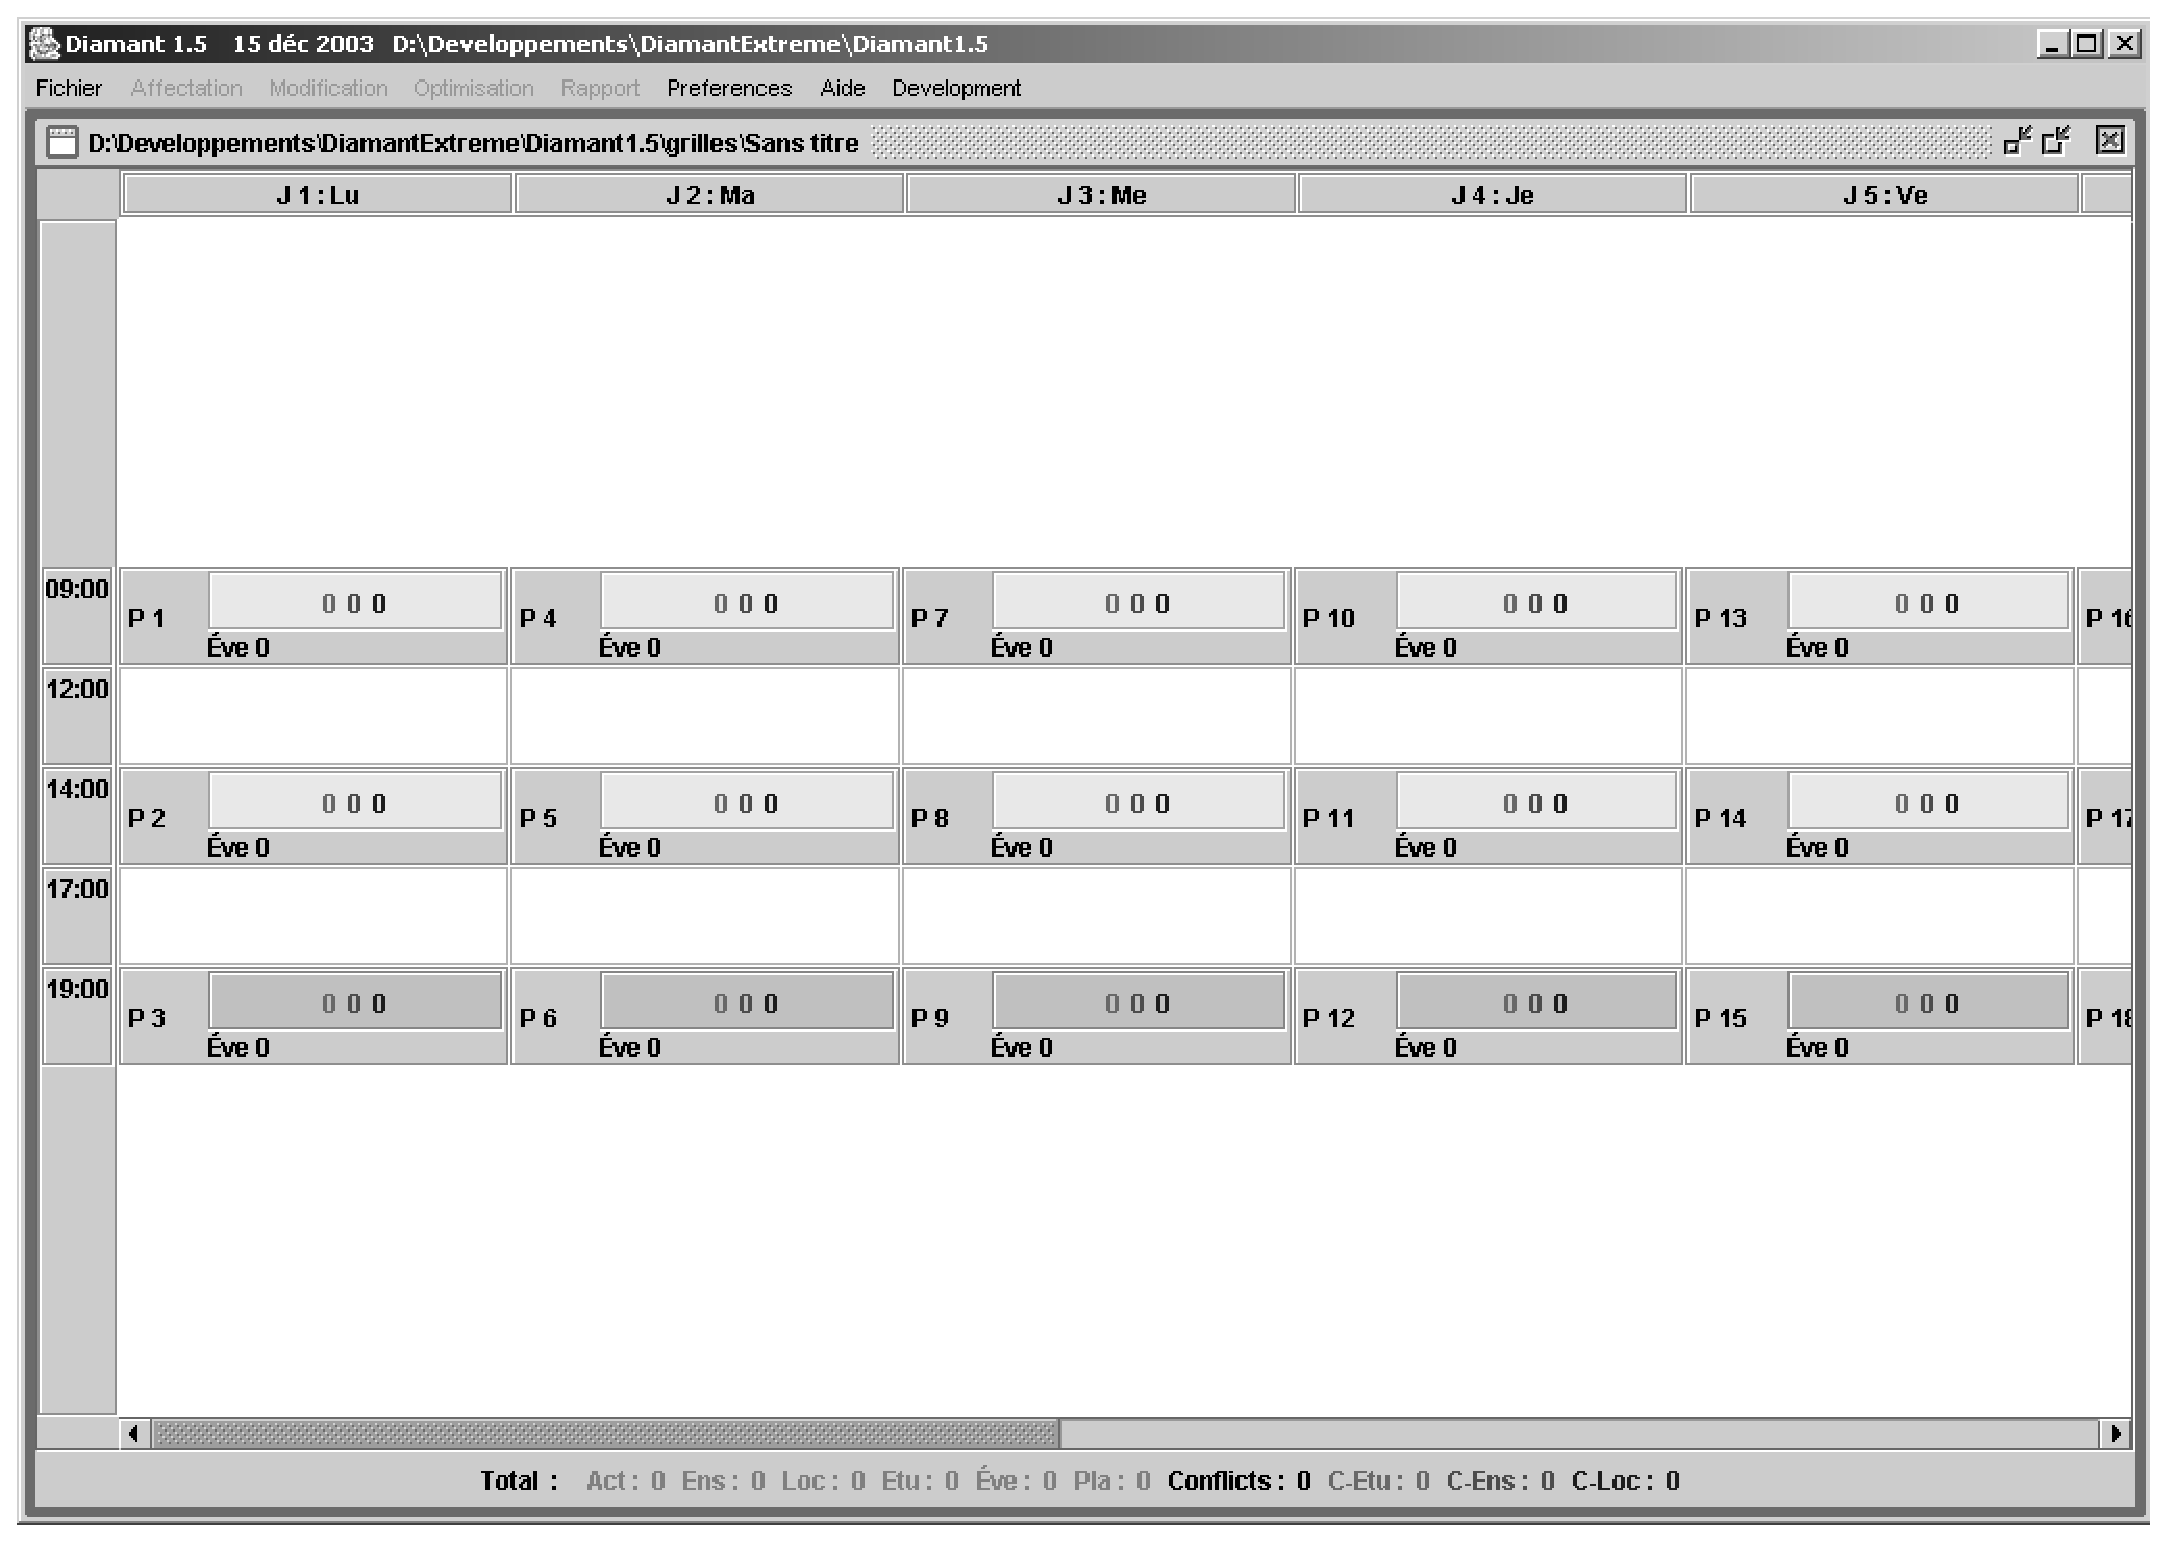
\includegraphics[width=4.5in]{UserManualInputs/images/grilleexam.eps}
    \caption{Grille horaire d'examen}\label{grilleexam}
  \end{center}
\end{figure}

    \item Aller au menu \textbf{\emph{Fichier}} et s�lectionner le menu \textbf{\emph{D�finir fichiers � importer}}. Une bo�te de dialogue comme celle de la Figure \ref{defautoimport}  doit appara�tre. Rep�rer l'endroit o� chacun des fichiers est localis�, puis cliquer sur le bouton \textbf{\emph{OK}}. Une nouvelle fen�tre se pr�sentera afin de vous permettre d'enregistrer la configuration des fichiers que vous venez de faire.

Il est recommand� d'enregistrer cette configuration en utilisant un nom de fichier unique et repr�sentatif.

Exemple: choisissez le nom de fichier \emph{H04exam} pour \emph{Hiver 2004 horaire d'examen} et le fichier cr�� sera \emph{H04exam.dim}. L'extension \textbf{\emph{.dim}} est rajout� automatiquement.

    \item Aller au menu \textbf{\emph{Fichier}} et s�lectionner le menu \textbf{\emph{Importer automatiquement}}.
    Une boite de dialogue appara�tra et vous permettra de choisir le fichier \textbf{\emph{.dim}} de �configuration de fichiers�
    pr�c�demment cr�� � partir de la fonction  \textbf{\emph{D�finir fichiers � importer}}
    (dans l'exemple pr�c�dent il s'agit du fichier \emph{H04exam.dim}).
    Cliquer � pr�sent sur le bouton \textbf{\emph{Importation de fichiers}},
    toutes vos donn�es (cours, �tudiants, enseignants et locaux) seront charg�es dans le logiciel et
    pr�tes � �tre modifi�es.
\end{enumerate}

� partir de cette �tape, la construction de l'horaire � proprement parler peut commencer. Il est vivement recommand� de lancer l'\textbf{\emph{Affectation initiale}} � partir du menu \textbf{\emph{Optimisation}} avant de poursuivre la production de l'horaire. Lancer l'\textbf{\emph{Affectation initiale}} � cette �tape ex�cuterait les fonctionnalit�s suivantes:

\begin{enumerate}
    \item Suppression des activit�s de nature 2, seulement les activit�s de nature 1 seront conserv�es pour l'horaire.
    \item Suppression des groupes aux activit�s en poss�dant plusieurs, un seul groupe sera conserv� pour l'horaire (le premier groupe ou \emph{groupe A}).
    \item Suppression des �v�nements aux activit�s en poss�dant plusieurs, un seul �v�nement sera conserv� pour l'horaire.
    \item Modification de la disponibilit� des enseignants afin de les rendre tous disponibles.
    \item Modification de la disponibilit� des locaux afin de les rendre tous disponibles.
\end{enumerate}

Exemple: Pour construire l'horaire d'examen d'une activit� (GEI200) poss�dant 2 natures (GEI200.1 et GEI200.2), chaque nature poss�dant 2 groupes (GEI200.1.A, GEI200.1.B et GEI200.2.A, GEI200.2.B), chaque groupe poss�dant 2 �v�nements (GEI200.1.A.1, GEI200.1.A.2, GEI200.1.B.1, GEI200.1.B.2 et GEI200.2.A.1, GEI200.2.A.2, GEI200.2.B.1, GEI200.2.B.2). La suppression de nature 2, de groupes et d'�v�nements par l'affectation initiale permettrait d'obtenir, pour l'activit� GEI200, un seul �v�nement devant servir � l'horaire d'examen, en l'occurrence GEI200.1.A.1.

Cette affectation initiale permettrait donc d'�purer les donn�es et d'initialiser le logiciel de sorte � pouvoir faire des modifications sur les donn�es et observer imm�diatement les repercussions sur l'horaire.

La pr�paration de l'horaire �tant achev�e, nous pouvons � pr�sent passer � la phase de modification et d'�puration de donn�es (phase 2). Il est cependant n�cessaire de noter que cette phase peut avoir lieu avant ou apr�s la phase de construction � proprement parler (phase 3), mais nous recommandons de la faire avant la phase 3 afin de travailler une bonne fois pour toute sur des donn�es propres (�pur�es).

\subsection{Modification et �purations des donn�es}

Le but de cette �tape est de permettre de construire l'horaire uniquement � partir de donn�es propres. Cette modification et/ou �puration peut se faire sur les activit�s, les �v�nements, les groupes d'�tudiants, les enseignants ou les locaux. 

\begin{itemize}
    \item Modifier une activit� en cliquant sur le menu \textbf{\emph{Affectation}} et le sous menu \textbf{\emph{Activit�s}} pour voir appara�tre la \emph{liste des activit�s} (voir figure \ref{listacte}) ou alors cliquer sur le menu \textbf{\emph{Affectation}} et le sous menu \textbf{\emph{�v�nements}} pour voir appara�tre la \emph{liste des �v�nements} (voir figure \ref{listeevente}).\\

� partir de la fen�tre \emph{liste des �v�nements}, vous pouvez s�lectionner un ou plusieurs �v�nements et les faire passer de la colonne \emph{fig�s} (les �v�nements sont plac�es et fig�es dans la grille horaire) � \emph{plac�s} (les �v�nements sont plac�es dans la grille horaire) ou de la colonne \emph{plac�s} � \emph{non plac�s} (les �v�nements ne sont pas encore plac�es dans la grille horaire) et vice-versa. 

    \begin{figure}[h]
      % Requires \usepackage{graphicx}
      \begin{center}
        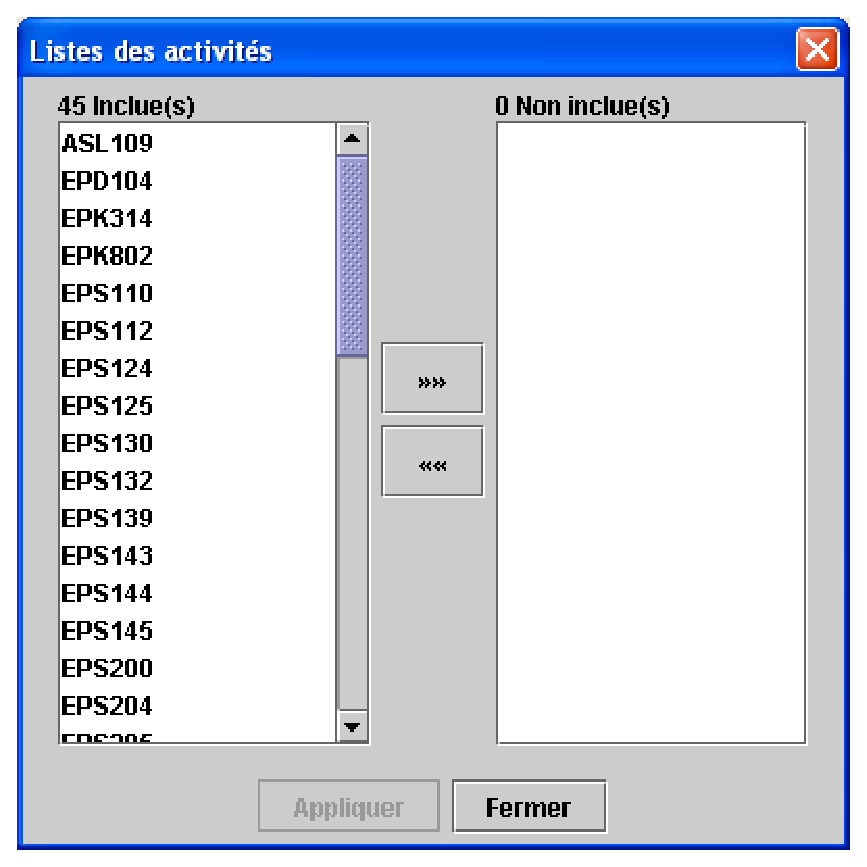
\includegraphics[width=2.5in]{UserManualInputs/images/listeact.eps}
        \caption{Liste des activit�s}\label{listacte}
      \end{center}
    \end{figure}

� partir de la fen�tre \emph{liste des activit�s}, vous pouvez s�lectionner une ou plusieurs activit�s et les faire passer de la colonne \emph{inclue(s)} � \emph{non inclue(s)} (non inclue(s)= les activit�s ne seront pas utilis�es dans la construction de l'horaire) et vice-versa. \\

    \begin{figure}[h]
      % Requires \usepackage{graphicx}
      \begin{center}
        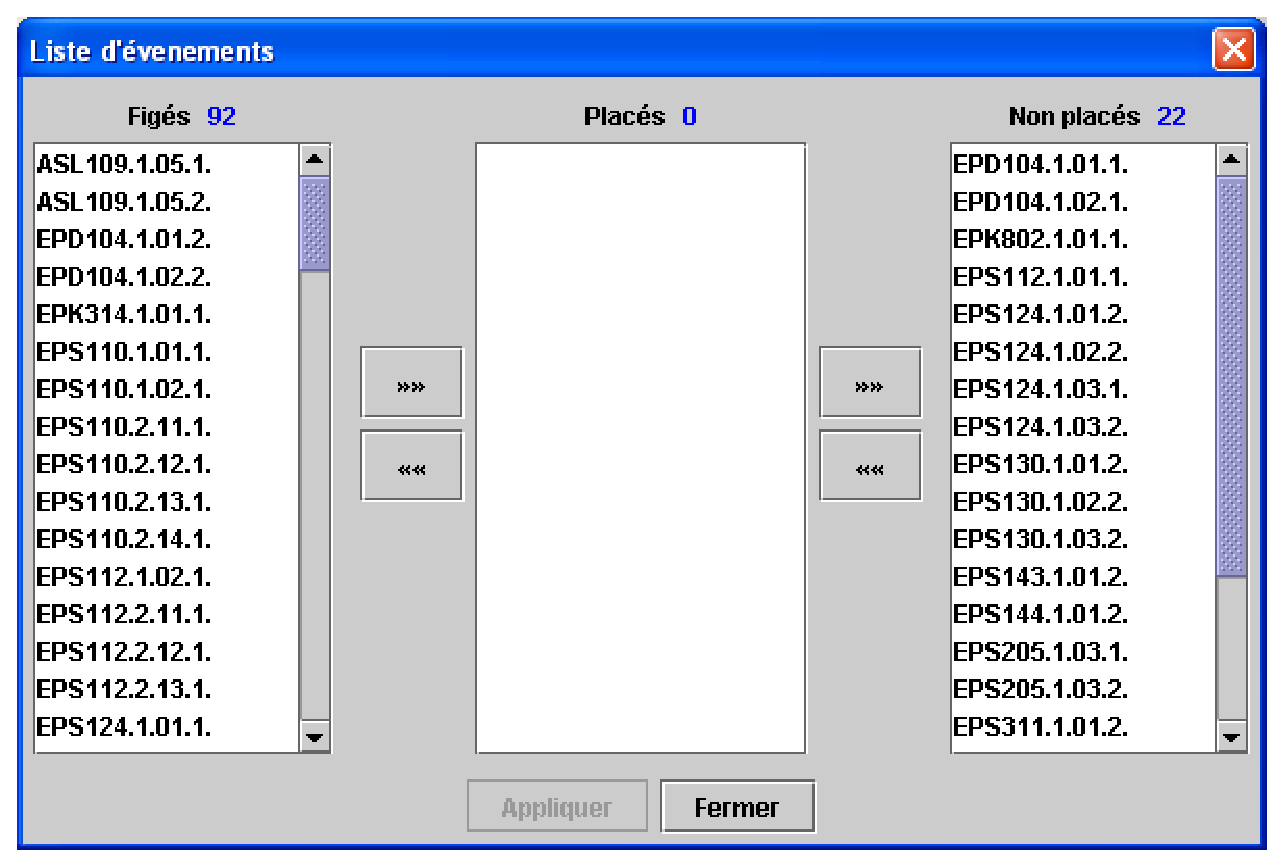
\includegraphics[width=2.5in]{UserManualInputs/images/listeevent.eps}
        \caption{Liste des �v�nements}\label{listeevente}
      \end{center}
    \end{figure}
   

� partir de l'une ou l'autre des fen�tres, double-cliquer sur l'activit� ou l'�v�nement � modifier pour faire appara�tre le dialogue d'\emph{affectation d'�v�nements} (voir figure \ref{evente}). Il vous est possible de modifier, � partir de cette fen�tre d'\emph{affectation d'�v�nements}, le jour et l'heure de d�but de l'�v�nement, l'enseignant, le local, de placer ou figer l'�v�nement.

    \begin{figure}[h]
      % Requires \usepackage{graphicx}
      \begin{center}
        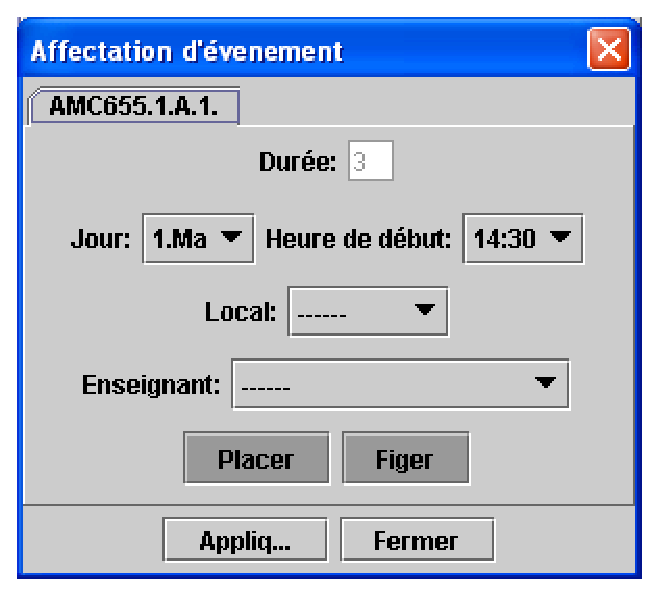
\includegraphics[width=2.5in]{UserManualInputs/images/event.eps}
        \caption{Affectation d'�v�nement}\label{evente}
      \end{center}
    \end{figure}
    
Cliquer sur \textbf{\emph{Appliquer}} pour valider les changements et Cliquer sur \textbf{\emph{Fermer}} pour fermer la fen�tre.\\
    
\item Modifier la disponibilit� d'un enseignant en cliquant sur le menu \textbf{\emph{Affectation}} et le sous menu \textbf{\emph{Enseignants}} pour voir appara�tre la fen�tre de la figure \ref{enseignante}. En s�lectionnant une zone correspondant au jour et � l'heure que vous souhaitez modifier. Une zone s�lectionn�e appara�t en fonc� et indique que l'enseignant y est disponible.
 
    \begin{figure}[h]
      % Requires \usepackage{graphicx}
      \begin{center}
        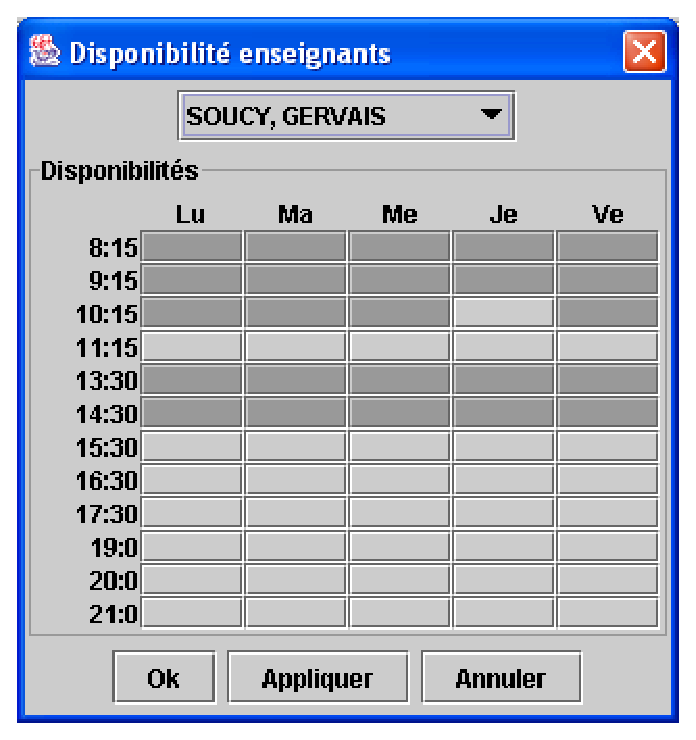
\includegraphics[width=2.5in]{UserManualInputs/images/enseignant.eps}
        \caption{Disponibilit� des enseignants}\label{enseignante}
      \end{center}
    \end{figure}

Cliquer sur \textbf{\emph{Appliquer}} pour accepter et effectuer les changements et Cliquer sur \textbf{\emph{Ok}} pour accepter, effectuer les changements et fermer la fen�tre.    \\

    \item Modifier la disponibilit� d'un local en cliquant sur le menu \textbf{\emph{Affectation}} et le sous menu \textbf{\emph{Locaux}} pour voir appara�tre la fen�tre de la figure  \ref{locale}. En s�lectionnant une zone correspondant au jour et � l'heure que vous souhait� modifier. Une zone s�lectionn�e appara�t en fonc� et indique que le local y est disponible. 

    \begin{figure}[h]
      % Requires \usepackage{graphicx}
      \begin{center}
        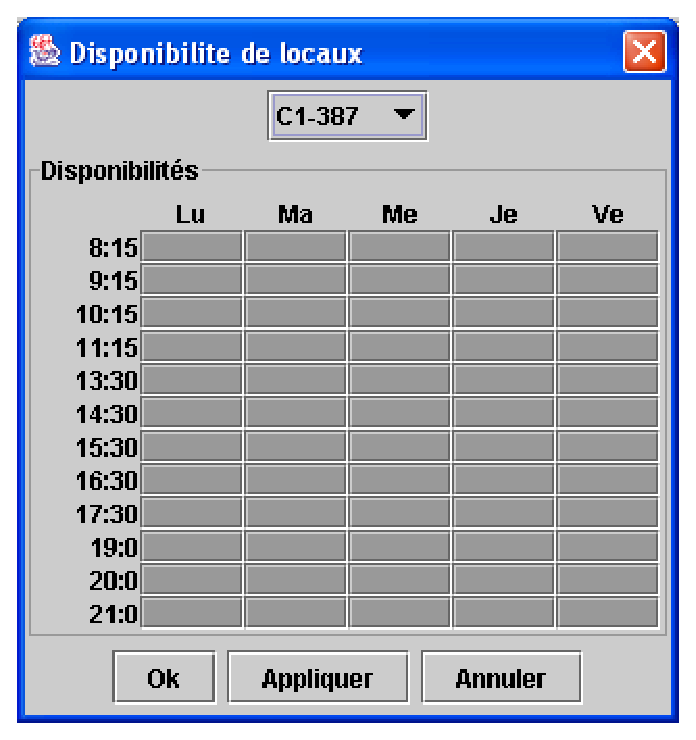
\includegraphics[width=2.5in]{UserManualInputs/images/local.eps}
        \caption{Disponibilit� des locaux}\label{locale}
      \end{center}
    \end{figure}

Cliquer sur \textbf{\emph{Appliquer}} pour accepter et effectuer les changements et Cliquer sur \textbf{\emph{Ok}} pour accepter, effectuer les changements et fermer la fen�tre.\\
        
 \end{itemize}    

\subsection{Construction de l'horaire}

Il est vivement recommand� de commencer cette �tape en lan�ant l'\textbf{\emph{affectation initiale}} � partir du menu \textbf{\emph{Optimisation}} (si cela n'a pas �t� pr�c�demment fait � la fin de la phase de pr�paration de l'horaire - section \ref{finprepae}) avant de poursuivre la production de l'horaire. La description des commandes ex�cut�es par l'affectation manuelle est faite � la section \ref{finprepae}.

Une fois l'affectation initiale effectu�e, l'�tape suivante consiste � lancer le sous menu \textbf{\emph{Construire l'horaire}} � partir du menu \textbf{\emph{Optimisation}}, afin de laisser le logiciel placer automatiquement dans la grille horaire les �v�nements (ceux qui n'ont pas encore �t� plac�s dans la grille horaire) respectant toutes les contraintes sp�cifi�es et ne cr�ant aucun nouveau conflit (conflits d'enseignants, conflits d'�tudiants et conflits de locaux).

La modification des contraintes � respecter par \dx{} lors de la construction automatique de l'horaire se fait en lan�ant le sous-menu \textbf{\emph{Options Conflits}} � partir du menu \textbf{\emph{Pr�f�rences}} pour faire appara�tre la fen�tre d'option de conflits (voir figure \ref{conf}). Cette fen�tre permet de modifier plusieurs param�tres, � savoir:

\begin{figure}[h]
      % Requires \usepackage{graphicx}
      \begin{center}
        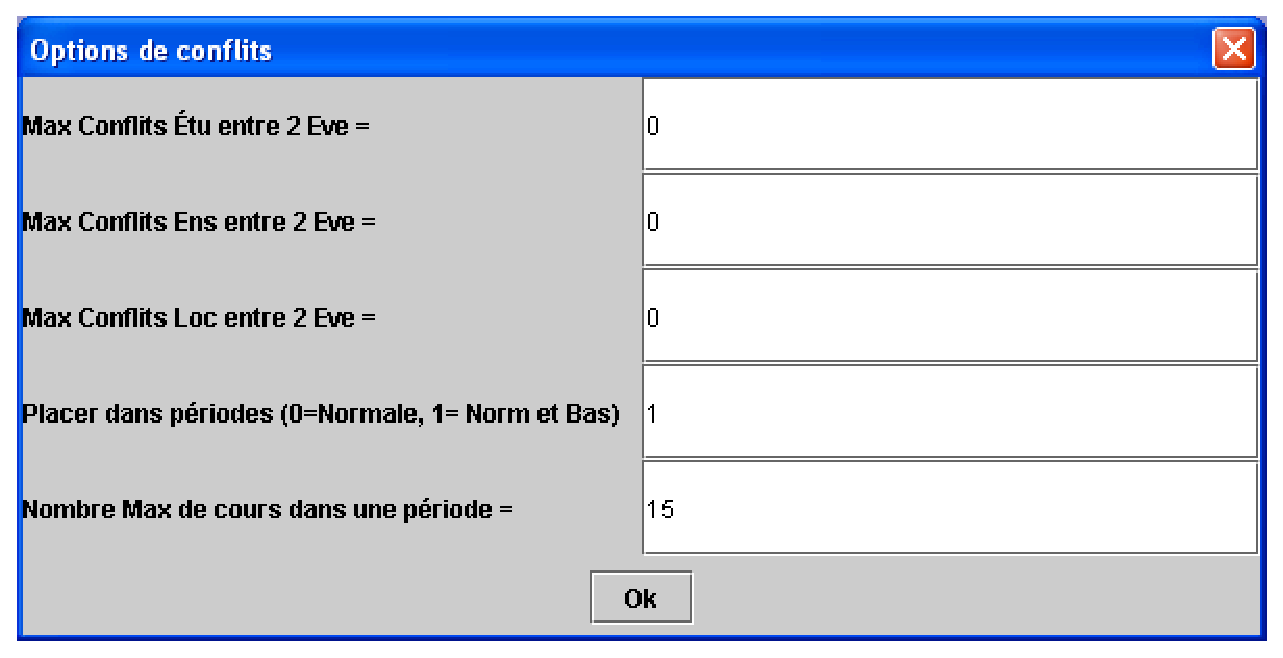
\includegraphics[width=3.5in]{UserManualInputs/images/optionconflict.eps}
        \caption{Contraintes � respecter}\label{conf}
      \end{center}
    \end{figure}

\begin{itemize}
    \item \emph{Max Conflits �tu entre 2 Eve}: ce param�tre permet de fixer le nombre maximal de conflits d'�tudiants admissible entre deux �v�nements.
    \item \emph{Max Conflits Ens entre 2 Eve}: ce param�tre permet de fixer le nombre maximal de conflits d'enseignants admissible entre deux �v�nements.
    \item \emph{Max Conflits Loc entre 2 Eve}: ce param�tre permet de fixer le nombre maximal de conflits de locaux admissible entre deux �v�nements.
    \item \emph{Placer dans p�riodes (0=normale, 1=normale et basse, 2=normale, basse et nulle)}: ce param�tre permet de sp�cifier les types de p�riodes (normale, basse, nulle) de la grille horaire dans lesquels un �v�nement peut �tre plac�.
    \item \emph{Nombre Max de cours dans une p�riode}: ce param�tre permet de sp�cifier le nombre maximal d'�v�nements pouvant �tre plac�s dans une m�me p�riode de la grille horaire.
\end{itemize}    

Il est possible de modifier les contraintes et lancer ensuite la construction de l'horaire afin que le logiciel  utilise les nouvelles contraintes pour placer les �v�nements qu'il n'a pas pu pr�c�demment placer; tout ceci de fa�on it�rative jusqu'� obtention d'un r�sultat paraissant satisfaisant aux yeux de l'utilisateur.

Si malgr� les it�rations, l'horaire construit n'est pas satisfaisant, il existe un certain nombre d'outils permettant de raffiner manuellement l'horaire.

\section{Raffinement de l'horaire}
Le raffinement de l'horaire propose � travers certains outils (affectation manuelle, rapport), les voies et moyens d'am�lioration de l'horaire construit.

\subsection{Affectation manuelle}

L'affectation manuelle permet � l'utilisateur de placer individuellement les �v�nements dans la grille horaire. Elle se fait � partir de la fen�tre d'\textbf{\emph{Affection manuelle}} (voir figure \ref{man}) obtenue � partir du sous-menu \textbf{\emph{Affectation manuelle}} du menu \textbf{\emph{Affectation}}.

    \begin{figure}[h]
      % Requires \usepackage{graphicx}
      \begin{center}
        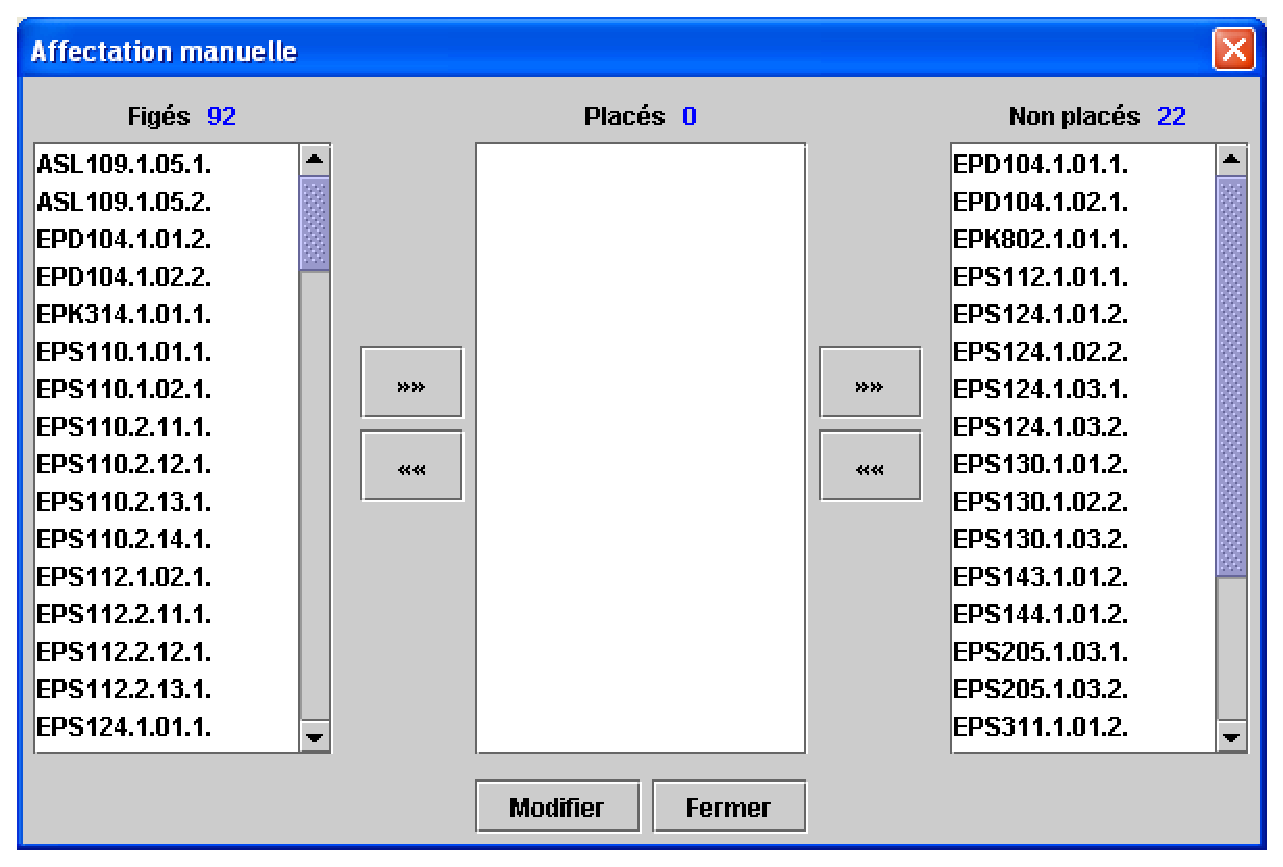
\includegraphics[width=3.5in]{UserManualInputs/images/manualaffect.eps}
        \caption{Liste des �v�nements}\label{man}
      \end{center}
    \end{figure}

La fen�tre d'affectation manuelle offre deux possibilit�s d'utilisation:

\begin{enumerate}
    \item \textbf{Modification d'un �v�nement:} s�lectionner un �v�nement et cliquer sur le bouton \textbf{\emph{Modifier}} pour faire appara�tre le dialogue d'\emph{affectation d'�v�nements} (voir figure \ref{evente}). Il vous est possible de modifier, � partir de cette fen�tre d'\emph{affectation d'�v�nements}, le jour et l'heure de d�but de l'�v�nement, l'enseignant, le local, de placer ou figer l'�v�nement.
    \item \textbf{Recherche de potentiels conflits:} pour rechercher les potentiels conflits g�n�r�s par un �v�nement, double-cliquer sur l'�v�nement en question pour voir appara�tre une nouvelle grille horaire (voir figure \ref{man1}) vous informant sur les conflits que peut g�n�r� l'�v�nement dans chaque p�riode de la grille horaire. \\

Une repr�sentation par les couleurs, de la grille horaire d'affectation manuelle, a �t� adopt�e afin de vous permettre, d'un seul coup d'oeil, de rep�rer les p�riodes de potentiels conflits (couleur rouge), les p�riodes dans lesquelles l'�v�nement peut �tre plac� sans g�n�rer de conflits (couleur par d�faut de la p�riode), et la ou les p�riodes dans lesquelles l'�v�nement est plac� (s'il �tait pr�c�demment plac� dans le grille - couleur verte).

    \begin{figure}[h]
      % Requires \usepackage{graphicx}
      \begin{center}
        \includegraphics[width=4.0in]{UserManualInputs/images/manualaffectres.eps}
        \caption{Grille horaire d'affectation manuelle}\label{man1}
      \end{center}
    \end{figure}

\end{enumerate}    

\subsection{Rapports}

%\chapter{Description des menus, des dialogues et des fen�tres}

\section{DESCRIPTION DES MENUS}


\begin{description}
    \item[Fichier :] permet de faire appel aux fonctions classiques relatives aux fichiers : Nouveau
projet, Nouveau, Ouvrir, Fermer, Enregistrer, Enregistrer sous, Importer manuellement,
D�finir le fichier Import Auto, Importer automatiquement, Exporter et Quitter.
    \item[Affichage :] permet de faire appel aux fonctions n�cessaire � l'affichage des fen�tres associ�es � un projet d'horaire.
    \item[Affectation :] permet d'affecter (fixer) certains choix relatifs � la construction d'un horaire, par exemple, un �tudiant dans un groupe donn� ou une activit� � une p�riode d�termin�e, etc. Contient aussi les menus qui permettent la construction automatique optimis�e d'un horaire.
    \item[Rapport :] permet de faire appel aux fonctions qui donnent acc�s aux rapports et de les sauvegarder comme des fichiers � texte �.
    \item[Pr�f�rences :] permet le changement de certains param�tres du programme.
    \item[Fen�tre :] Permet d'ouvrir une fen�tre de listes de conflits pr�c�demment ouverte.
    \item[Aide :] permet d'obtenir de l'information sur le logiciel ainsi que de l'aide.
\end{description}    
 

%  
% 
% 
% 
% 


\appendix
\chapter{Description des fichiers d'entr�e de \diamant{}}

\diamant{} version 1.0 et 1.5 utilise les fichiers suivantes qui
viennent du STI (Syst�me informatique central)~:

\begin{enumerate}
    \item �tudiants.
    \item Instructeurs.
    \item Activit�s.
\end{enumerate}

Le fichier de locaux est produit par l'utilisateur. Les premiers
fichiers ont un format tr�s rigides. Le nombre de caract�res et
leur position est � respecter obligatoirement.

Les indexes de cha�nes de caract�res commencent � \verb!0!.



\section{Fichier d'�tudiants}

C'est l'un des fichiers pr�alables � la construction de l'horaire.

\subsection{Exemple des donn�es qu'il contient}

\begin{verbatim}
001342
009008132035030720003LUPIEN MY05
CTB301101 GIS251102 GIS351102 GRH111101 GRH332101
009011991290000520021AUDET FRE05
CTB341101 FEC111102 FEC444101 GIS114101 MAR221107
009022232035010720003AUDET STE05
CTB443102 CTB451101 CTB513101 CTB563101 CTB613102
009027042035010720003VEILLEUX 05
CTB443101 CTB451102 CTB513102 CTB563101 CTB613102
009031242035010720003FAUCHER M05
\end{verbatim}

\subsection{Signification des donn�es}

Il existe trois types de lignes :

\begin{enumerate}
    \item nombre d'�tudiants dans le fichier;
    \item identification de l'�tudiant et nombre de cours qu'il prend;
    \item l'identification de cours que l'�tudiant suit.
\end{enumerate}

La structure du fichier :

\begin{enumerate}
\item Le chiffre du d�but du fichier $n$, \verb!001342!, nous indique
le nombre d'�tudiants contenus dans ce fichier. Il s'agit d'une ligne du premier type.
\item Ensuite il y a $n$ couples de lignes du type 2 et 3.
\end{enumerate}

La ligne de type 2 contient des chiffres et de lettres correspondant au num�ro
d'identification unique de l'�tudiant (� l'exception des deux derniers entiers de la ligne).
Ce num�ro d'identification renferme plusieurs informations
pertinentes. Soit :
\begin{itemize}
      \item Le matricule de l'�tudiant qui correspond aux huit premiers chiffres
      du num�ro d'identification (Indices 0 � 7).
       Dans notre exemple, \verb!00900813! pour l'�tudiant
       \verb!LUPIEN! et \verb!00901199! pour l'�tudiante \verb!AUDET!.
      \item Le programme auquel l'�tudiant appartient correspond ensuite aux six chiffres suivants.
      Soit \verb!203503! dans le cas du premier �tudiant (Indices 8 � 13).
     \item La version du programme que l'�tudiant suit correspond aux deux chiffres suivants.
     Soit \verb!07! dans le cas du premier �tudiant (Indices 14 � 15).
      \item Des informations sur l'admission de l'�tudiant sont donn�es par les cinq chiffres suivants.
       Les quatre premiers correspondent � l'ann�e d'admission tandis
       que le cinqui�me indique le trimestre d'admission.
        Soit \verb!20003! dans le cas du premier �tudiant (Indices 16 � 20).
    \item Suit ensuite neuf places pour indiquer le nom de famille
    de l'�tudiant suivit d'un espace et de son pr�nom (coup� apr�s neuf espaces) (Indices 21 � 29).
    Soit, dans notre exemple, \verb!LUPIEN MY! dans le cas de la premi�re �tudiante.
    \item Vient alors un chiffre de deux caract�res qui correspond en fait au nombre de cours que suit l'�tudiant.
    \verb!05! dans le cas du premier �tudiant (Indices 30 � 31).
\end{itemize}


Finalement, nous avons la liste des activit�s suivies par
l'�tudiant. Soit \verb!CTB301101! dans le cas du premier �tudiant.
Les 6 premiers caract�res (\verb!GEI441!) correspondent au num�ro
du cours. Le septi�me caract�re (\verb!1!) correspond � la nature
du cours (1=Le�on Magistrale et 2=autre). Le 2 derniers caract�res
(\verb!01!) sont facultatifs dans un fichier et ils correspondent
au groupe d'activit� dans lequel l'�tudiant est assign�.

\subsection{D�finition des champs}
xxx

\section{Fichier d'instructeurs}

Ce fichier contient les donn�es de disponibilit�s des enseignants.

\subsection{Exemple des donn�es qu'il contient}


\begin{verbatim}
116
ATALLA, NOUREDDINE
1 1 1 1 5 5 5 5 5 5 5 5 5 5
5 5 5 5 5 5 5 5 5 5 5 5 5 5
5 5 5 5 5 5 5 5 5 5 5 5 5 5
5 5 5 5 5 5 5 5 5 5 5 5 5 5
1 1 1 1 5 5 5 5 5 5 5 5 5 5
BALLIVY, G�RARD
1 1 1 1 5 1 1 1 1 1 5 5 5 5
1 1 1 1 5 1 1 1 1 1 5 5 5 5
1 1 1 1 5 1 1 1 1 1 5 5 5 5
1 1 1 5 5 1 1 1 1 5 5 5 5 5
1 1 1 1 5 1 1 1 5 5 5 5 5 5
\end{verbatim}


\subsection{Signification des donn�es}

Il existe trois types de lignes :

\begin{enumerate}
    \item le nombre d'enseignants dans le fichier;
    \item l'identification de l'enseignant;
    \item tableau de disponibilit�.
\end{enumerate}

La structure du fichier :
Le fichier commence avec un chiffre repr�sentant le nombre d'enseignants qu'il contient. Vient ensuite une suite de blocs contenant le nom d'un professeur suivi de sa disponibilit�. Le nom de l'enseignant ne doit pas exc�der trente caract�res. Les \texttt{1} signifient que l'enseignant est disponible � la p�riode correspondante et les 5 qu'il
ne l'est pas du tout.

Chaque ligne repr�sente une journ�e, en commen�ant par lundi, jusqu'� vendredi. Chaque colonne correspond � une heure
dans la journ�e (8h30, 9h30, 10h30, 11h30, 12h30, 13h30, 14h30, 15h30, 16h30, 17h30,  18h30, 19h00, 20h00 et 21h00).
 Les disponibilit�s sont ainsi connues entre 8h30 et 21h00.


\section{Fichier d'activit�s}

Ce fichier contient des informations concernant les cours offerts � une session. Nous y retrouvons la liste des
activit�s associ�es, l'agencement du cours, le nom de l'enseignant qui le donnera, etc.
C'est un fichier pr�alable � la construction de l'horaire.

\subsection{Exemple des donn�es qu'il contient}


\begin{verbatim}

ADM1111  A
1
1
LUC LAJOIE


 2
 2 1
 2 1 4 2
1 1
C1-387 C1-380
0 0
0 0
0 0

ADM1111  B
1
1
R�AL CAOUETTE


 1
 3
 2 12
1
C1-387
0
0
0

AMC6401  A
1
1
FADI AL-HAMED


 2
 2 1
 2 1 4 2
1
D73020
0
0
0
\end{verbatim}


\subsection{Signification des donn�es}
\begin{description}
\item [Ligne blanche] la premi�re ligne du fichier est une ligne blanche.
\item [ADM1111   A]   C'est le sigle du cours (\texttt{ADM1111 A} pour la le�on magistrale du cours
\texttt{ADM111} avec le groupe \texttt{A}).
\item [1]  Ensuite, vient le nombre un ou z�ro. \texttt{1} nous indique alors que le cours est actif, contrairement � \texttt{0}.
\item [1]  Cet entier nous donne le nombre de \textit{fiches professeurs}. Ceci est en fait le nombre d'activit�s
associ�es � ce cours (LM, ED, LAB, etc.).
\item [LUC LAJOIE] Puis, commence alors la description d'une des fiches. Sur cette premi�re ligne, on y retrouve le nom de ou des enseignants de la premi�re fiche (avec une limite de 3 noms).
\item [2] le nombre de blocs de p�riodes s�par�es de la premi�re fiche (ex: si nous avons deux heures de cours coll�es � trois endroits diff�rents dans l'horaire, l'entier sera 3).
\item [2 1] Nous avons une suite de nombre qui correspond � la dur�e de chacun des blocs pr�vus � la ligne pr�c�dente. Dans ce cas-ci, la dur�e du premier bloc est de deux p�riodes alors que la dur�e du deuxi�me est de seulement une p�riode.
\item [2 1 4 2] On a une autre liste d'entiers repr�sentant le jour et l'heure de chacun des blocs pr�c�dents. Ici, \texttt{2 1} nous indique que le premier bloc a lieu le mardi � 8h30 alors que \texttt{4 2} nous apprends que le deuxi�me bloc est le jeudi � 9h30.
\item [1 1] Cette ligne nous indique si le local de cette activit� est fix� ou non. Effectivement, un \texttt{1} nous dit qu'il l'est alors qu'un \texttt{0} nous indique le contraire.
\item [C1-387 C1-380] Sur cette ligne, nous avons les nom des locaux pour le premier et le deuxi�me bloc respectivement.
\item [0 0] Puis vient le type de locaux requis par cette activit� (voir le manuel d'utilisation de \saphir{} \cite{ruben94})
\item [0 0] Idem (voir le manuel d'utilisation de \saphir{} \cite{ruben94})
\item [0 0] Et finalement, cette rang�e permet de savoir si le bloc � �t� pr�affect� � l'horaire \texttt{(1)} ou non \texttt{(0)}.
\item [ADM1111  B] Puis on recommence pour la deuxi�me activit� ainsi de suite...
\end{description}

\section{Fichier de locaux}

\subsection{Exemple des donn�es qu'il contient}

\begin{verbatim}
//Facult� des sciences;

//Nom du local;Capacit�;Fonction;Liste des caract�ristiques;Notes;

D13012;32;211;08,11,14,57;laboratoire de chimie;
D13013;40;211;08,11,57;laboratoire de chimie;
D13014;20;211;08,44,57;laboratoire de chimie;
D13016;18;211;08,57;laboratoire de chimie;
\end{verbatim}

\subsection{Signification des donn�es}

\begin{description}
    \item[Premi�re ligne] cette ligne repr�sente la facult�.
    \item[Deuxi�me ligne] cette ligne d�crit le fichier.
    \item[Troisi�me ligne] cette ligne est blanche.
    \item[Quatri�me ligne] cette ligne d�crit l'organisation des informations sur les locaux.
    \item[Cinqui�me ligne] cette ligne est blanche
    \item[De la sixi�me � la derni�re ligne ] chaque ligne donne les informations sur un local. Chaque information est s�par�e par un \texttt{;} et est d�crite comme suit:
    \begin{itemize}
        \item Le nom du local \texttt{D13012} pour le premier local.
        \item La capacit� du local \texttt{32} pour le premier local.
        \item La fonction du local \texttt{211} pour le premier local (voir le manuel d'utilisation de \saphir{} \cite{anoyme94})
        \item Liste des caract�ristiques 08,11,14,57 pour le premier local (voir le manuel d'utilisation de \saphir{} \cite{anoyme94}). Il peut y avoir plusieurs caract�ristique, elles seront s�par�es par des \texttt{,}
        \item La description du local \texttt{laboratoire de chimie} pour le premier local.
    \end{itemize}
\end{description}

\chapter{Description du fichier $.dia$ de sauvegarde de projet de \diamant{} 1.5}

La sauvegarde d'un projet sous \dx{} se fait essentiellement �
travers un fichier $.dia$. Dans ce fichier sont stock�s diff�rents
types d'information du projet. Les types sont s�par�s entre eux
par le s�parateur suivant~:

\verb!=================================!

 Ce fichier comporte six
types de donn�es structur�s comme suit~:


\begin{enumerate}
    \item Version du logiciel,
    \item Emplacement de la grille horaire utilis�e,
    \item Donn�es relatives aux enseignants,
    \item Donn�es relatives aux locaux,
    \item Donn�es relatives aux activit�s,
    \item Donn�es relatives aux �tudiants.
\end{enumerate}

\section{Version du logiciel}
Le premier type de donn�es du fichier $.dia$ est une cha�ne de
caract�res sur une ligne indiquant la version du logiciel.

\section{Emplacement de la grille horaire}
Le second type de donn�es du fichier $.dia$ est une cha�ne de
caract�res indiquant l'emplacement du fichier $.xml$ contenant la
structure de la grille horaire.

\section{Donn�es relatives aux enseignants}
Le troisi�me type de donn�es du fichier $.dia$ repr�sente la
disponibilit� des enseignants, les donn�es sont d�crits dans la
section \ref{instructor}. Mais dans la sauvegarde le nombre de
p�riodes de la disponibilit� est �gal au nombre de p�riodes de la
grille horaire.

\section{Donn�es relatives aux locaux}
Le quatri�me type de donn�es du fichier $.dia$ repr�sente les
caract�ristiques des locaux (voir section \ref{room} pour plus de
details), ainsi que leur disponibilit� (nouveaux champs rajout�s �
ceux d�crits � la section \ref{room}).

\subsection{Exemple des donn�es qu'il contient}

\begin{verbatim}
C2-1007;21;212;08,11,14,57;laboratoire de chimie;1 1 1 1 1 1 1 1 1
1 1 1, 1 1 1 1 1 1 1 1 1 1 1 1,1 1 1 1 1 1 1 1 1 1 1 1,1 1 1 1 1 1
1 1 1 1 1 1, 1 1 1 1 1 1 1 1 1 1 1 1; C1-2018;10;212;11;Mat�riaux
composites;1 1 1 1 1 1 1 1 1 1 1 1, 1 1 1 1 1 1 1 1 1 1 1 1,1 1 1
1 1 1 1 1 1 1 1 1,1 1 1 1 1 1 1 1 1 1 1 1, 1 1 1 1 1 1 1 1 1 1 1
1; C1-3014;25;211;11;Laboratoire m�catronique;1 1 1 1 1 1 1 1 1 1
1 1, 1 1 1 1 1 1 1 1 1 1 1 1,1 1 1 1 1 1 1 1 1 1 1 1,1 1 1 1 1 1 1
1 1 1 1 1, 1 1 1 1 1 1 1 1 1 1 1 1; C1-3027;15;211;11;Petit
laboratoire de communication pour �lect; 1 1 1 1 1 1 1 1 1 1 1 1,1
1 1 1 1 1 1 1 1 1 1 1,1 1 1 1 1 1 1 1 1 1 1 1, 1 1 1 1 1 1 1 1 1 1
1 1,1 1 1 1 1 1 1 1 1 1 1 1;
\end{verbatim}

\subsection{Signification des donn�es}
Chaque ligne est compos�e de six types d'informations:
    \begin{itemize}
        \item Le nom du local \texttt{C2-1007} pour le premier local.
        \item La capacit� du local \texttt{21} pour le premier local.
        \item La fonction du local \texttt{212} pour le premier
        local.
        \item Liste des caract�ristiques 08,11,14,57 pour le premier local.
        Il peut y avoir plusieurs caract�ristiques, elles seront s�par�es par des \texttt{,}
        \item La description du local \texttt{laboratoire de chimie} pour le premier local.
        \item La disponibilit� du local. Une s�quence du genre \verb!1 1 1 1 1 1 1 1 1 1 1 1!
        repr�sente la disponibilit� du local durant une journ�e.
        Le s�parateur \verb!,! s�pare la disponibilit� d'une journ�e � celle d'une autre.
        \item Le nombre de
p�riodes de la disponibilit� est �gal au nombre de p�riodes de la
grille horaire.
    \end{itemize}

\section{Donn�es relatives aux activit�s}

Le cinqui�me type de donn�es du fichier $.dia$  contient des
informations concernant les cours offerts � une session. Nous y
retrouvons la liste des activit�s associ�es, l'agencement du
cours, le nom de l'enseignant qui le donnera, etc.

\subsection{Exemple des donn�es qu'il contient}


\begin{verbatim}
AMC6552  01
1
1
NEAIME, SAMIR F. ;
1
3
3.3.1
0
------
1
1
1 ;1
AMC9001  01
1
1
ST-AMANT, REN� ; ST-AMANT, REN� ;
2
3 3
3.1.1 3.2.1
1 1
C1-5012 C1-5012
0 0
0  0
1 1 ;1 1
\end{verbatim}


\subsection{Signification des donn�es}

Il existe douze types de lignes :

\begin{enumerate}
    \item L'identification du cours;
    \item L'�tat du cours (actif ou inactif);
    \item Le nombre d'activit�s associ�es au cours;
    \item Le nom de l'enseignant du cours. Si l'activit� a plus d'un bloc, il y'aura autant d'enseignants qu'il y'aura de blocs et les noms des enseignants seront s�par�s par des �~;~�;
    \item Le nombre de blocs d'activit�;
    \item La dur�e de chacun des blocs identifi�s � la ligne pr�c�dente;
    \item La p�riode � laquelle le ou les blocs sont plac�s. La p�riode est sous la forme $a.b.c$ o� $a$ repr�sente le jour, $b$ repr�sente la s�quence et $c$ repr�sente la p�riode;
    \item l'�tat du local affect� � chaque unit� (fix� ou non fix�);
    \item le nom du local assign� � chaque unit�;
    \item le type de locaux requis � chaque unit�;
    \item le type de locaux requis � chaque unit�;
    \item Cette ligne poss�de deux types d'informations s�par�es par le �~;~�. Le premier type d'information indique l'�tat fig� (1) ou non (0) du bloc, tandis que le second type indique l'�tat plac� (1) ou non (0) du bloc.
\end{enumerate}

\section{Donn�es relatives aux �tudiants}

Le sixi�me type du fichier $.dia$ repr�sente les choix de cours des �tudiants.

\subsection{Exemple des donn�es qu'il contient}

\begin{verbatim}
004
022515472365000420031MERCIER B06
GEL410101;0 GEN400101;0 GIF400101;0 GIF420101;0 GIF430101;0 GIF440101;0
022519582145000520031BERGERON 06
GEL400101;0 GEL410101;0 GEL420101;0 GEL430101;0 GEL440101;0 GEN400101;0
915965442120000520023MARTINEAU05
GCH106101;0 GCH106201;0 GCH205101;0 GCH205201;0 GCH210101;0
965509672135000620012NGUYEN TH07
GCI200101;0 GCI200201;0 GCI220101;1 GCI220201;0 GCI600101;0
GCI600201;0 GIN600101;0
\end{verbatim}

\subsection{Signification des donn�es}

Il existe trois types de lignes :

\begin{enumerate}
    \item Nombre d'�tudiants dans le fichier;
    \item Identification de l'�tudiant et nombre de cours qu'il prend;
    \item L'identification de cours que l'�tudiant suit. Cette identification poss�de deux types d'informations s�par�es par le �~;~�.
    \begin{itemize}
    \item Le premier type, soit \verb!GEL410101! dans le cas du premier �tudiant.
    Les 6 premiers caract�res (\verb!GEL410!) correspondent au num�ro
    du cours. Le septi�me caract�re (\verb!1!) correspond � la nature ou type d'activit�
    du cours (1=Le�on Magistrale et 2=autre). Le 2 derniers caract�res
    (\verb!01!) correspondent au groupe d'activit� dans lequel l'�tudiant est assign�.
    \item Le second type indique si l'�tudiant est fig� (1) ou non (0) dans le groupe auquel il est assign�.
    \end{itemize}
\end{enumerate}



\printindex

%\part{Une partie}
%\include{revue}
%\include{theorie}

%\part{Derni�re partie}
%\chapter{Conclusion}

Bla bla bla bla bla.

Bla bla bla bla bla.

%\chapter*{Glossaire}

Bla bla bla bla bla.

Bla bla bla bla bla.

%\chapter*{Index}

A
AAA
ABC.

B
Bla bla bla bla bla.

%\include{formules}
\end{articleDX}
\end{document}
